\documentclass{vkr}
\usepackage[english, russian]{babel} % переносы
\usepackage{graphicx} % для вставки картинок
\graphicspath{{images/}} % путь к изображениям

%\usepackage{xltabular} % для вставки таблиц

\newcommand{\centrow}{\centering\arraybackslash} % командой \centrow можно центрировать одну ячейку (заголовок) в столбце типа X или p, оставив в оcтальных ячейках другой тип выравнивания
\newcommand{\finishhead}{\endhead\hline\endlastfoot}

% из-за того что babel переопределяет имена заголовков
\addto\captionsrussian{\renewcommand{\figurename}{Рисунок}}



% Режим шаблона (должен быть включен один из трех)
\ВКРtrue
%\Практикаtrue
%\Курсоваяtrue

\newcommand{\Дисциплина}{<<Проектирование и архитектура программных систем>>} % для курсовой
\newcommand{\КодСпециальности}{09.03.04} % Курсовая
\newcommand{\Специальность}{Программная инженерия} % Курсовая
\newcommand{\Тема}{Разработка web-сайта «Русатом – Аддитивные технологии» на платформе} % ВКР Курсовая
\newcommand{\ТемаВтораяСтрока}{1С-Битрикс}
\newcommand{\ГдеПроводитсяПрактика}{Юго-Западном государственном университете} % для практики
\newcommand{\РуководительПрактПредпр}{Куркина А. В.} % для практики
\newcommand{\ДолжнРуководительПрактПредпр}{директор} % для практики
\newcommand{\РуководительПрактУнивер}{Чаплыгин А. А.} % для практики
\newcommand{\ДолжнРуководительПрактУнивер}{к.т.н. доцент} % для практики
\newcommand{\Автор}{И. И. Иванов}
\newcommand{\АвторРод}{Иванова И.И.}
\newcommand{\АвторПолностьюРод}{Иванова Ивана Ивановича} % для практики
\newcommand{\Шифр}{хх-хх-хххх}
\newcommand{\Курс}{4} % для практики
\newcommand{\Группа}{ПО-92б}
\newcommand{\Руководитель}{А. А. Чаплыгин} % для ВКР и курсовой
\newcommand{\Нормоконтроль}{А. А. Чаплыгин} % для ВКР
\newcommand{\ЗавКаф}{А. В. Малышев} % для ВКР
\newcommand{\ДатаПриказа}{«07» апреля 2023~г.} % для ВКР
\newcommand{\НомерПриказа}{1505-с} % для ВКР
\newcommand{\СрокПредоставления}{«13» июня 2023~г.} % для ВКР, курсового

\begin{document}
\maketitle
\ifПрактика{}\else{
   \newpage
\begin{center}
\large\textbf{Минобрнауки России}

\large\textbf{Юго-Западный государственный университет}
\vskip 1em
\normalsize{Кафедра программной инженерии}
\vskip 1em

\begin{flushright}
\begin{tabular}{p{.4\textwidth}}
\centrow УТВЕРЖДАЮ: \\
\centrow Заведующий кафедрой \\
\hrulefill \\
\setarstrut{\footnotesize}
\centrow\footnotesize{(подпись, инициалы, фамилия)}\\
\restorearstrut
«\underline{\hspace{1cm}}»
\underline{\hspace{3cm}}
20\underline{\hspace{1cm}} г.\\
\end{tabular}
\end{flushright}
\end{center}
\vspace{1em}
\begin{center}{ЗАДАНИЕ НА ВЫПУСКНУЮ КВАЛИФИКАЦИОННУЮ РАБОТУ
  ПО ПРОГРАММЕ БАКАЛАВРИАТА}\end{center}
\vspace{1em}
{\parindent0pt
  Студента \АвторРод, шифр\ \Шифр, группа \Группа
  
1. Тема «\Тема\ \ТемаВтораяСтрока» утверждена приказом ректора ЮЗГУ от \ДатаПриказа\ № \НомерПриказа.

2. Срок предоставления работы к защите \СрокПредоставления

3. Исходные данные для создания программной системы:

3.1. Перечень решаемых задач:}

\renewcommand\labelenumi{\theenumi)}

\begin{enumerate}
\item проанализировать IT-инфраструктуру предприятия;
\item  разработать концептуальную модель системы управления IT-ин\-фра\-струк\-турой предприятия на основе подхода к управлению и организации ИТ-услуг ITSM;
\item спроектировать программную систему управления IT-ин\-фра\-струк\-турой предприятия;
\item сконструировать и протестировать программную систему управления IT-инфраструктурой предприятия.
\end{enumerate}

{\parindent0pt
  3.2. Входные данные и требуемые результаты для программы:}

\begin{enumerate}
\item Входными данными для программной системы являются: данные
справочников комплектующих, конфигураций, ПО, критериев качества SLA,
ИТ-услуг, департаментов компании; технические данные ИТ-ресурсов; данные входящих заявок на ИТ-ресурсы; данные запросов поставщикам на комплектующие.
\item Выходными данными для программной системы являются: сформированные заявки на обслуживание ИТ-ресурсов; сформированные запросы на
закупку комплектующих; сведения о выполненных работах по заявкам; статусы заявок; выходные отчеты (инфографика) – по качеству услуг, по состоянию ИТ-ресурсов, по деятельности ИТ-отдела, по стоимости обслуживания
ИТ-ресурсов, воронка заявок.
\end{enumerate}

{\parindent0pt

  4. Содержание работы (по разделам):
  
  4.1. Введение
  
  4.1. Анализ предметной области
  
4.2. Техническое задание: основание для разработки, назначение разработки,
требования к программной системе, требования к оформлению документации.

4.3. Технический проект: общие сведения о программной системе, проект
данных программной системы, проектирование архитектуры программной системы, проектирование пользовательского интерфейса программной системы.

4.4. Рабочий проект: спецификация компонентов и классов программной системы, тестирование программной системы, сборка компонентов программной системы.

4.5. Заключение

4.6. Список использованных источников

5. Перечень графического материала:

\списокПлакатов

\vskip 2em
\begin{tabular}{p{6.8cm}C{3.8cm}C{4.8cm}}
Руководитель ВКР & \lhrulefill{\fill} & \fillcenter\Руководитель\\
\setarstrut{\footnotesize}
& \footnotesize{(подпись, дата)} & \footnotesize{(инициалы, фамилия)}\\
\restorearstrut
Задание принял к исполнению & \lhrulefill{\fill} & \fillcenter\Автор\\
\setarstrut{\footnotesize}
& \footnotesize{(подпись, дата)} & \footnotesize{(инициалы, фамилия)}\\
\restorearstrut
\end{tabular}
}

   \abstract{РЕФЕРАТ}

Объем работы равен \formbytotal{lastpage}{страниц}{е}{ам}{ам}. Работа содержит \formbytotal{figurecnt}{иллюстраци}{ю}{и}{й}, \formbytotal{tablecnt}{таблиц}{у}{ы}{}, \arabic{bibcount} библиографических источников и \formbytotal{числоПлакатов}{лист}{}{а}{ов} графического материала. Количество приложений – 2. Графический материал представлен в приложении А. Фрагменты исходного кода представлены в приложении Б.

Перечень ключевых слов: веб-приложение, домашние животные, социальная сеть.

Объектом разработки является веб-приложение <<Социомаркет для владельцев домашних животных>>, представляющее собой платформу, на которой владельцы домашних животных могут находить и предлагать различные услуги и товары. Это приложение будет интегрировано в популярные социальные сети и мессенджеры для облегчения доступа и использования.

Целью работы является создание удобной и функциональной платформы, которая помогает владельцам домашних животных находить необходимые услуги и товары, а также предоставлять свои услуги другим пользователям. Это достигается путем разработки веб-приложения с интуитивно понятным интерфейсом и полезными функциональностями.

В процессе разработки программно-информационной системы были использованы методы объектно-ориентированного программирования. Серверная часть системы разработана на основе .NET Core, а клиентская часть -\- на Angular. База данных системы построена на PostgreSQL, что обеспечивает её надежность и эффективность.

Для работы приложения на стороне пользователя необходимо мобильное устройство или компьютер с доступом в интернет с установленным браузером. Приложение оптимизировано для работы как в современных так и в более старых версиях браузеров и не требует значительных ресурсов аппаратного обеспечения.

Для размещения программы на стороне сервера необходим компьютер с операционной системой Windows 10, процессор с тактовой частотой не ниже 1.6 ГГц, ОЗУ 1024 Мб. Для обеспечения стабильной работы базы данных необходимо место на жестком диске 1 ГБ или больше. Для работы серверной части приложения так же потребуется установка программной платформы .NET 6.0, а для клиентской части -\- Node.js.

Состояние системы: веб-приложение находится на стадии внедрения и доступно для использования всеми заинтересованными сторонами. Оно предоставляет уникальную возможность для владельцев домашних животных взаимодействовать и обмениваться услугами и товарами в удобной и безопасной среде.

\selectlanguage{english}
\abstract{ABSTRACT}
  
The volume of work is \formbytotal{lastpage}{page}{}{s}{s}. The work contains \formbytotal{figurecnt}{illustration}{}{s}{s}, \formbytotal{tablecnt}{table}{}{s}{s}, \arabic{bibcount} bibliographic sources and \formbytotal{числоПлакатов}{sheet}{}{s}{s} of graphic material. The number of applications is 2. The graphic material is presented in annex A. The layout of the site, including the connection of components, is presented in annex B.

List of keywords: web application, pets, social network.

The object of development is the web application <<Sociomarket for pet owners>>, which is a platform on which pet owners can find and offer various services and products. This application will be integrated into popular social networks and instant messengers for ease of access and use.

The goal of the work is to create a convenient and functional platform that helps pet owners find the necessary services and products, as well as provide their services to other users. This is achieved by developing a web application with an intuitive interface and useful functionality.

In the process of developing the software information system, object-oriented programming methods were used. The server part of the system is developed based on .NET Core, and the client part is based on Angular. The system database is built on PostgreSQL, which ensures its reliability and efficiency.

To operate the application on the user side, you need a mobile device or computer with Internet access and a browser installed. The application is optimized to work in both modern and older versions of browsers and does not require significant hardware resources.

To host the program on the server side, you need a computer with the Windows 10 operating system, a processor with a clock frequency of at least 1.6 GHz, and 1024 MB of RAM. To ensure stable operation of the database, a hard disk space of 1 GB or more is required. To operate the server part of the application, you will also need to install the .NET 6.0 software platform, and for the client part -\- Node.js.

System Status: The web application is in the implementation stage and is available for use by all interested parties. It provides a unique opportunity for pet owners to interact and exchange services and goods in a convenient and safe environment.

\selectlanguage{russian}
}\fi
\tableofcontents
\section*{ОБОЗНАЧЕНИЯ И СОКРАШЕНИЯ}

БД -\- база данных.

СУБД -\- система управления базами данных.

ООП -\- объектно-ориентиронное программирование.

EF Core -\- Entity Framework Core, система управления объектно-реляционным отображением для .NET Core.

ORM -\- Object-Relational Mapping, технология программирования, позволяющая использовать базы данных с объектно-ориентированным подходом.

Angular -\- фреймворк для разработки веб-приложений.

HTML -\- HyperText Markup Language, язык гипертекстовой разметки.

JavaScript -\- язык программирования для веб-разработки.

SCSS -\- Sassy CSS, препроцессор, расширяющий возможности CSS.

UI -\- User Interface, пользовательский интерфейс.

REST API -\- Representational State Transfer Application Programming Interface, интерфейс программирования приложений, использующий архитектурный стиль REST.

CRUD -\- Create, Read, Update, Delete, основные операции для работы с данными.

MVC -\- Model-View-Controller, архитектурный шаблон проектирования.
\ifПрактика{}\else{\section*{ВВЕДЕНИЕ}
\addcontentsline{toc}{section}{ВВЕДЕНИЕ}

Цифровизация и инновации в сфере услуг для домашних животных значительно расширяют горизонты для предпринимателей и пользователей. Настоящая дипломная работа посвящена разработке веб-приложения «Социомаркет для владельцев домашних животных», направленного на улучшение доступности и качества услуг для владельцев домашних животных.

\emph{Цель настоящей работы} -\- разработка веб-приложения, объединяющего владельцев домашних животных и предоставляющих услуги для них. 

Для достижения цели настоящей работы были поставлены \emph{следующие задачи:}

\begin{itemize}
    \item провести анализ предметной области;
    \item разработать пользовательский интерфейс клиентской части приложения;
    \item спроектировать архитектуру и разработать серверную часть приложения;
    \item реализовать клиент-серверное взаимодействие частей приложений.
\end{itemize}

\emph{Структура и объем работы.} Данный отчет представляет собой выпускную квалификационную работу, которая включает в себя введение, четыре основных раздела, заключение, список использованных источников и два приложения. Общий объем текста этой работы составляет \formbytotal{page}{страниц}{у}{ы}{}.

\emph{Во введении} определена цель и поставлены задачи, описана структура работы и представлено краткое содержание каждого из разделов.

\emph{В первом разделе} подробно рассмотрены актуальные аспекты рынка услуг для животных, рассмотрено воздействие цифровой трансформации на обслуживание, а также проанализированы инновационные тенденции и технологии, связанные с предоставлением услуг временного содержания животных.

\emph{Во втором разделе} сформулированы основные требования к разработке веб-приложения. В нем содержатся цели и задачи проекта, а также требования пользователя к интерфейсу. Кроме того, данный раздел охватывает различные функциональные аспекты и обсуждает архитектуру системы.

\emph{В третьем разделе} объясняется выбор используемых технологий проектирования, таких как .NET Core, Entity Framework Core, PostgreSQL и Angular. Также в этом разделе осуществляется проектирование пользовательского интерфейса и предоставление описания классов системы.

\emph{В четвертом разделе} данной работы представлен подробный список классов и их методов, которые были использованы в процессе разработки сайта. Кроме того, в этом разделе проводится детальное тестирование разработанного веб-сайта, с целью проверки его функциональности и стабильности.

\emph{В заключении} преподносятся основные выводы и результаты, полученные в ходе разработки проекта.

В приложении А представлен графический материал.
В приложении Б представлены фрагменты исходного кода серверной части приложения. 
В приложении В представлены фрагменты исходного кода клиентской части приложения. }\fi
\section{Анализ предметной области}

\subsection{Исследование предметной области}

Современный мир цифровых трансформаций и социальных изменений вносит заметные инновации в сферу услуг для домашних животных. Наблюдается укрепление трендов, направленных на улучшение качества жизни домашних питомцев, что стимулирует появление новых услуг и продуктов. Особенно важным становится принцип индивидуального подхода к уходу за животными, подразумевающий применение интегрированных решений, учитывающих потребности как животных, так и их владельцев.

Ветеринарные услуги, груминг и передержка животных активно адаптируют новейшие технологии и методологии. В частности, расширение сферы телемедицины в ветеринарии позволяет владельцам получать консультации специалистов на расстоянии. Важным становится также предоставление информационных ресурсов для поддержки и обучения владельцев животных, улучшая тем самым общий уровень ухода за питомцами.

Рынок товаров для домашних животных, включающий корма, одежду, аксессуары и игрушки, также испытывает расширение. Развитие электронной торговли и смарт-технологий, например, интеллектуальных кормушек и трекеров активности, способствует усилению динамики роста в этой области.

Таким образом, рынок услуг и товаров для домашних животных превращается в сложную и разнообразную сферу, требующую инновационных подходов для удовлетворения потребностей животных и их владельцев. Цифровые платформы и технологии занимают ключевую роль, обеспечивая удобство, доступность и качество услуг и продуктов.

\subsection{Роль цифровых платформ}

Применение цифровых технологий приводит к существенным изменениям в сегменте услуг для домашних животных, особенно в области временного содержания животных. Разнообразие предлагаемых услуг, от гостиниц для животных до индивидуальных услуг по уходу, становится доступным благодаря цифровой интеграции. Это упрощает процессы бронирования и управления услугами, увеличивая их доступность и прозрачность. Важность экологической устойчивости и этических стандартов в уходе за животными также возрастает.

Цифровые платформы предлагают широкий спектр онлайн-сервисов, от информационных порталов до комплексных приложений для бронирования и управления услугами. Это значительно упрощает поиск, бронирование и оплату услуг, включая:

\begin{itemize}
  \item Страхование домашних животных;
  \item Выездной груминг;
  \item Выгул собак;
  \item Услуги няни для котов;
  \item Консультации психолога для котов;
  \item Гостиницы для животных;
  \item Зоотакси;
  \item Фитнес и тренировки для собак;
  \item Телемедицина для животных.
\end{itemize}

Преимущества этих решений включают удобство доступа, возможность быстрого сравнения цен и услуг, а также получение обратной связи от пользователей. Однако существуют и определенные ограничения, такие как необходимость персонализации услуг в соответствии с индивидуальными потребностями животных, а также вопросы безопасности данных и зависимости от качества интернет-соединения.

Для эффективной работы цифровых платформ критично важно создать многофункциональную модель данных, охватывающую информацию о пользователях, поставщиках услуг, доступных услугах, ценах, расписании и отзывах. Это улучшит взаимодействие между пользователями и поставщиками и повысит уровень удовлетворенности клиентов.

<<Социомаркет для "владельцев домашних животных">> обладает рядом уникальных функций, предназначенных для удовлетворения потребностей владельцев домашних животных. Основные функции включают создание, редактирование, поиск и просмотр карточек с товарами и услугами. Это позволяет пользователям в полной мере управлять информацией о предлагаемых услугах, таких как:

\begin{itemize}
  \item Выездной груминг;
  \item Выгул собак;
  \item Временная передержка собак;
  \item Услуги няни для котов;
  \item Продажа животных.
\end{itemize}

Цифровые платформы, такие как <<Петбук>> и <<Петмир>>, выполняют ключевую роль в соединении владельцев домашних животных с поставщиками услуг. Они обеспечивают пользователей инструментами для сравнения цен, просмотра отзывов и участия в онлайн-сообществах. Разнообразие бизнес-моделей этих платформ, включая модели прямых продаж и подписок, способствует их эффективной монетизации.

\subsection{Технологии разработки веб-приложений}

Разработка серверной части веб-приложений включает в себя использование множества технологий и подходов. Среди основных можно выделить:

\begin{itemize}
  \item \textbf{SQL-ориентированные базы данных:} Эти базы данных, включая MySQL, PostgreSQL и Microsoft SQL Server, предпочтительны для систем с необходимостью сложных запросов и транзакционной целостности.
  \item \textbf{NoSQL базы данных,} включая MongoDB и Cassandra, используются для более гибкой структуры данных и лучшей масштабируемости.
\end{itemize}

Выбор .NET Core и Angular для разработки был обусловлен их гибкостью, масштабируемостью и удобством в сопровождении.
PostgreSQL выбран в качестве СУБД, т.к. позволяет эффективно обрабатывать большие объемы данных и сложные запросы, а также за поддержку JSON, что делает PostgreSQL идеальной СУБД для гибких веб-приложений.

\subsection{Анализ аудитории пользователей веб-приложений для владельцев домашних животных}

Аудитория веб-приложений для владельцев домашних животных представляет собой разнообразную группу, объединенную общей заботой о благополучии своих питомцев. Эта группа включает людей различных возрастных категорий, социально-экономических статусов и образовательных уровней, но с общими интересами в области ухода за животными и использования технологий для улучшения качества жизни своих питомцев.

\textbf{Демографические Характеристики:}
Большинство пользователей веб-приложений для домашних животных принадлежат к возрастной группе от 25 до 45 лет, активно используют цифровые технологии в повседневной жизни и часто ищут удобные и инновационные способы улучшения ухода за своими животными.

\textbf{Поведенческие Особенности:}
Пользователи часто ищут информацию о лучших практиках ухода за животными, сравнивают различные продукты и услуги, исследуют отзывы других пользователей и активно участвуют в онлайн-сообществах. Они предпочитают платформы, которые предлагают простой и интуитивно понятный интерфейс, а также ценят возможность получить персонализированные рекомендации.

\textbf{Потребности и Предпочтения:}
Важными факторами для пользователей являются надежность, безопасность и доступность услуг. Они ожидают высокого качества обслуживания, прозрачности цен и легкости доступа к услугам. Предпочтения включают разнообразие предлагаемых услуг, таких как онлайн-консультации ветеринаров, автоматизированные напоминания о медицинских процедурах и индивидуально подобранные программы питания и ухода за животными.

\textbf{Влияние на Дизайн и Функциональность Веб-Приложения:}
На основе анализа аудитории, разработка веб-приложения должна быть сфокусирована на создании удобного и функционального интерфейса, который облегчает навигацию и поиск информации. Важным аспектом является интеграция функций обратной связи и коммуникационных инструментов, позволяющих пользователям делиться опытом и получать поддержку. Внедрение аналитических инструментов для сбора данных о предпочтениях пользователей поможет в создании более персонализированных и целенаправленных предложений, тем самым повышая удовлетворенность и лояльность клиентов.

В заключение, аудитория веб-приложений для владельцев домашних животных требует комплексного подхода, который сочетает в себе удобство, информативность и возможность персонализации. Понимание их потребностей и предпочтений является ключом к разработке успешного и востребованного

\subsection{Перспективы развития}

В перспективе развития веб-приложения ключевым является масштабирование его возможностей. Для Angular-приложений это может включать применение ленивой загрузки модулей, оптимизацию производительности и улучшение пользовательского интерфейса. .NET приложения могут масштабироваться путем интеграции микросервисов, что позволяет разделить приложение на независимые компоненты, упрощая управление и обновление. В будущем можно рассмотреть интеграцию бэкенда в виде набора микросервисов, а фронтенда – как микрофронтенда, что обеспечит более гибкое управление ресурсами и улучшит масштабируемость приложения.

Сектор ветеринарной медицины и ухода за домашними животными переживает значительные трансформации благодаря технологическим инновациям. Прогресс в этой сфере включает использование передовых диагностических инструментов, роботизированных хирургических систем и искусственного интеллекта для диагностики, что позволяет повысить точность и эффективность медицинской помощи. Особое внимание уделяется генетическим тестам для определения наследственных заболеваний и разработке новых методов лечения, включая терапию стволовыми клетками и плазматерапию. Важной является интеграция ИИ для повышения точности диагностики и эффективности лечения в ветеринарной медицине.

\section{Техническое задание}
\subsection{Основание для разработки}

Полное наименование системы: <<Веб-приложение \textquotedbl Социомаркет для владельцев домашних животных \textquotedbl\ >>.
Основанием для разработки программы является приказ ректора ЮЗГУ от <<24>> ноября 2023 г. №5166-с <<Об утверждении тем выпускных квалификационных работ>>.

\subsection{Цель и назначение разработки}

Веб-приложение <<Социомаркет для владельцев домашних животных>> создается с целью объединения пользователей двух групп: владельцев домашних животных и лиц, предоставляющих услуги для домашних животных. Такими лицами могут являться владельцы интернет-магазинов, предприниматели или такие же пользователи.

Задачами данной разработки являются:
\begin{itemize}
\item создание каталогов с категориями карточек на сайте;
\item разработка клиентской части web-сайта;
\item создание каталогов с категориями карточек на сайте;
\item реализация формы создания и управления карточкой услуги;
\item создание удобного поиска по каталогам карточкам;
\item реализация взаимодействия между пользователями сайта;
\item разработка и развертывание инфраструктуры web-сайта и его базы данных на удаленном сервере;
\item разработка серверной части web-сайта;
\item разработка REST API для взаимодействия клиентской и серверной частей;
\item разработка базы данных.
\end{itemize}

Задачей разработки серверной части также является следования принципам, описанным в работе Марка Прайса <<C\# 9 и .NET 5. Разработка и оптимизация>> \cite{mark_price}.

\subsection{Требования пользователя к интерфейсу web-сайта}

Сайт должен включать в себя:
\begin{itemize}
    \item авторизацию;
    \item навигацию по разделам;
    \item разделение доступа к функционалу сайта для пользователя и лица предоставляющего услуги;
    \item поиск по пользователям и их товарам или услугам.
\end{itemize}


\subsection{Требования к программной системе веб-приложения <<Социомаркет>>}
\subsubsection{Требования к данным программной системы}
Система должна уметь эффективно обрабатывать данные пользователей, включая личную информацию, данные о питомцах, информацию о продуктах (товары и услуги). Необходимо обеспечить конфиденциальность и безопасность этих данных.
На рисунке  \ref{bd:image} представлена концептуальная модель данных программной системы в виде UML-диаграммы сущность-связь.

\begin{figure}[ht]
\centering
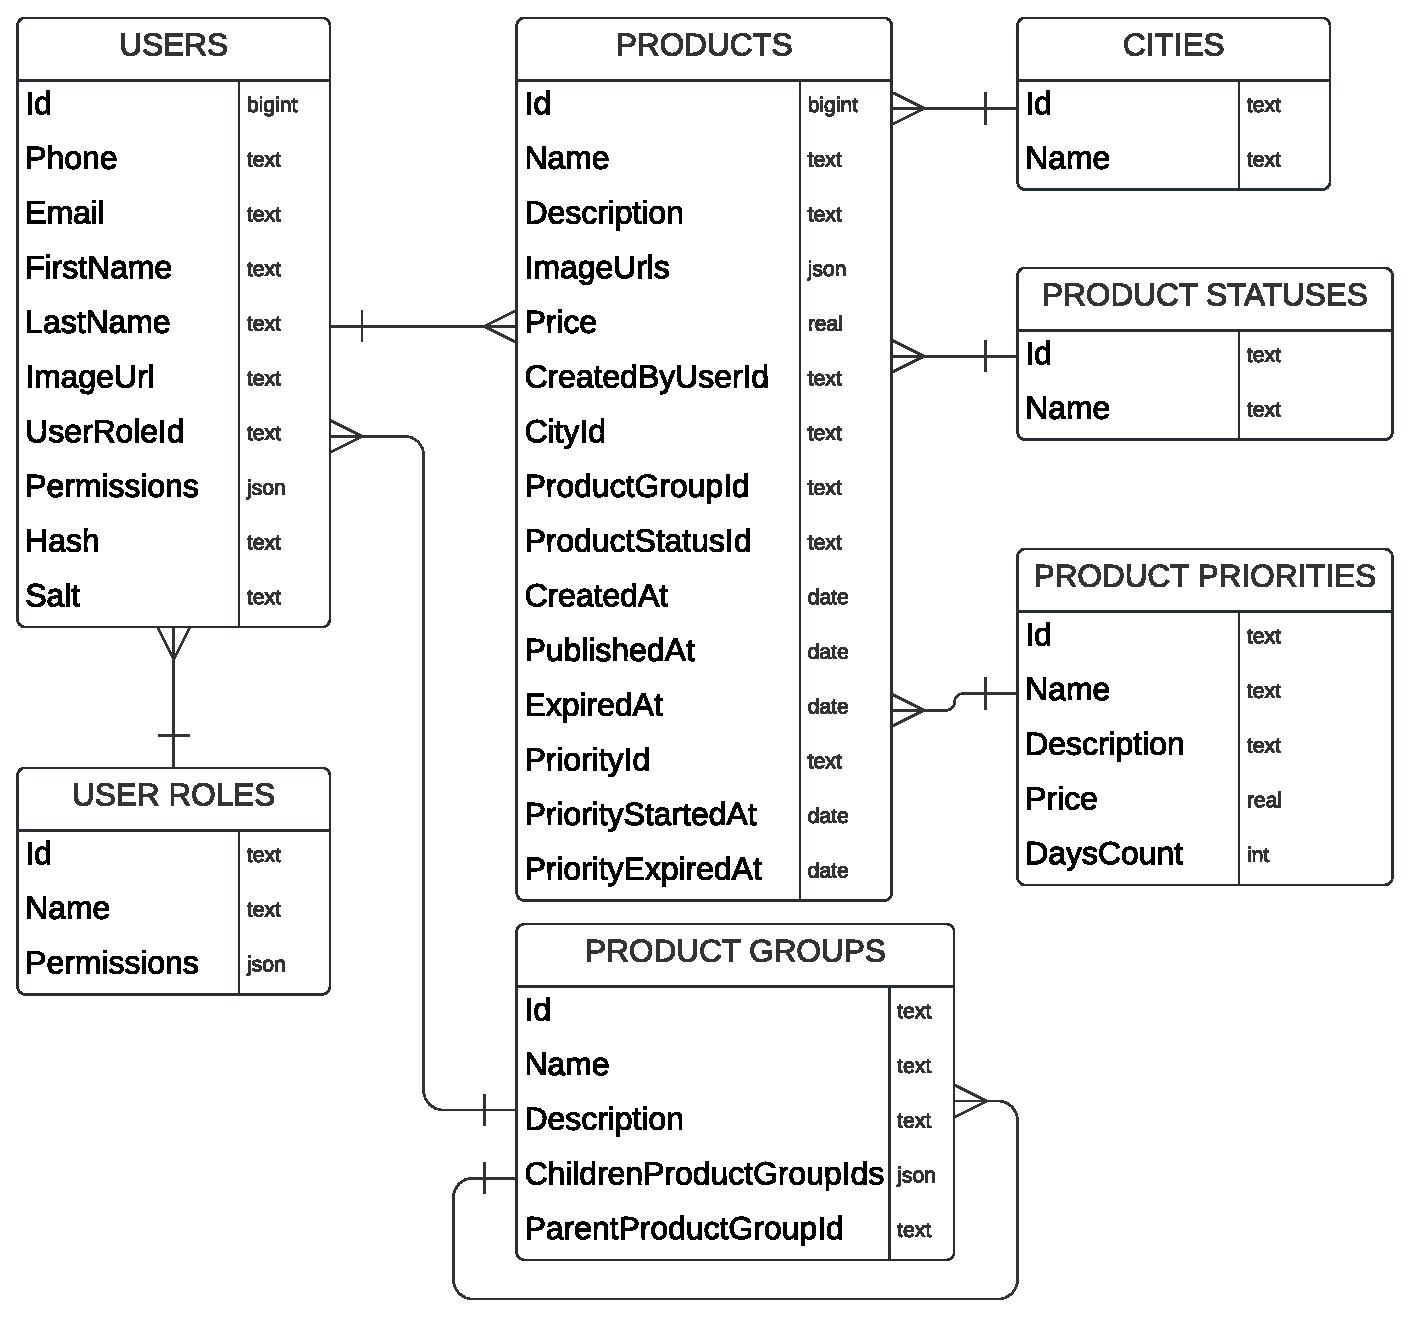
\includegraphics[width=1\linewidth]{bd}
\caption{Концептуальная модель данных}
\label{bd:image}
\end{figure}

В приведенной на рисунке \ref{bd:image} диаграмме сущность-связь представлены сущности и атрибуты, которые будут использоваться в программной системе.

Данные программной системы должны быть организованы таким образом, чтобы не разделять на 2 отдельные группы пользователей и лиц, предоставляющих услуги. Отличие между пользователями должно быть записано в атрибуте <<UserRole>> сущности <<User>>. Таким образом, в программной системе будет только одна сущность <<User>>, которая будет иметь атрибут <<UserRole>> со значениями <<SITTER>> и <<OWNER>>.
При проектировании модели данных также необходимо учесть то, что сущность <<Product>> представляет собой продукт, который может быть как товаром, так и услугой. Для этого не требуется никаких дополнительных атрибутов, так как сущность <<Product>> становится товаром или услугой в зависисмости от названия и описания карточки продукта.

\subsubsection{Архитектура системы} 
Серверная часть веб-приложения <<Социомаркет>> разработана на .NET Core, что отражает современные подходы в разработке программного обеспечения, описанные в <<C\# 9 и .NET 5. Разработка и оптимизация>> \cite{mark_price}. Клиентская часть, реализованная на Angular, взаимодействует с сервером через REST API. База данных построена на PostgreSQL и соответствует рекомендациям и методикам, изложенным в документации PostgreSQL \cite{postgresql}.

\subsubsection{Функциональные требования к программной системе}

На основании анализа предметной области, разрабатываемая программная система <<Социомаркет для владельцев домашних животных>> должна включать в себя следующие ключевые функциональные возможности:

\begin{itemize}
\item <<Регистрация с ролью: Клиент>>
\item <<Регистрация с ролью: Продавец>>
\item <<Поиск по карточкам>>
\item <<Просмотр карточек>>
\item <<Создать карточку>> -\- Предоставление функциональности для продавцов по созданию карточек, которые будут содержать всю необходимую информацию о предлагаемых товарах или услугах;
\item <<Редактировать карточку>> -\- Возможность для продавцов изменять содержимое ранее созданных карточек, чтобы информация оставалась актуальной;
\item <<Удалить карточку>> -\- Реализация опции удаления карточек для продавцов, позволяющая убирать предложения, которые более неактуальны или доступны.
\item <<Начать общение с другим пользователем о карточке>>
\end{itemize}

Эти требования отражают основные сценарии использования системы и направлены на создание удобного и эффективного сервиса для обоих классов пользователей: клиентов и продавцов.

На рисунке \ref{people:image} представлена диаграмма прецедентов, которая служит важным средством для систематизации функциональных требований и возможностей системы, выявляя ключевые сценарии использования. Диаграмма прецедентов изображает, как пользователи могут взаимодействовать с системой, а также помогает выявить набор основных функциональных возможностей, доступных пользователям. Каждый прецедент на диаграмме отражает отдельный путь взаимодействия в системе и представляет потенциальные действия, которые могут быть предприняты пользователями в различных ролях.

\begin{figure}[ht]
\centering
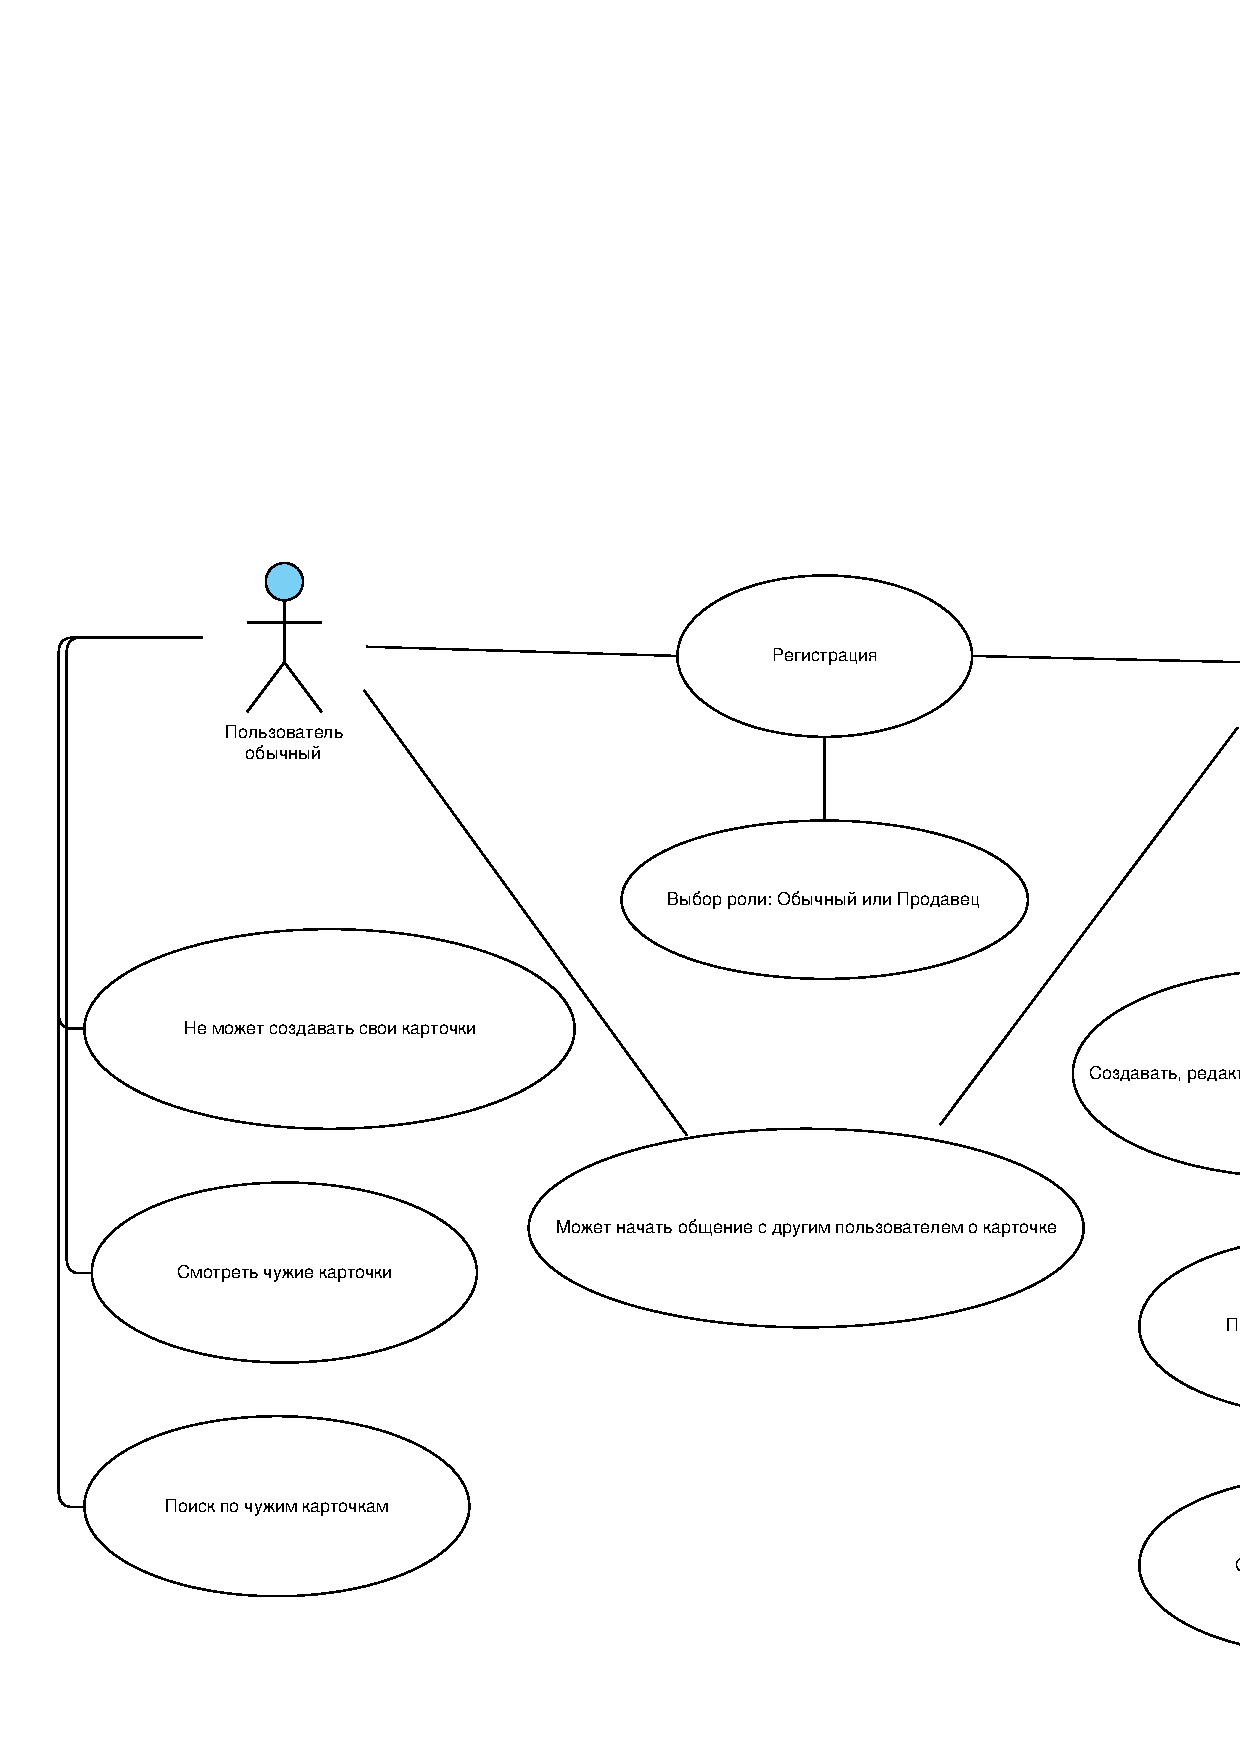
\includegraphics[width=1\linewidth]{people}
\caption{Диаграмма прецедентов}
\label{people:image}
\end{figure}

\subsubsection{Вариант использования <<Регистрация с ролью: Клиент>>}
Клиенты регистрируются в системе, предоставляя свои личные данные для создания профиля, что позволяет им пользоваться услугами платформы.

\subsubsection{Вариант использования <<Регистрация с ролью: Продавец>>}
Продавцы регистрируются в системе, указывая информацию о своих товарах и услугах, что дает им возможность размещать карточки товаров и услуг для просмотра и покупки клиентами.

\subsubsection{Вариант использования <<Поиск по карточкам>>}
Пользователи могут выполнять поиск карточек товаров и услуг с помощью ключевых слов и фильтров для нахождения наиболее подходящих предложений.

\subsubsection{Вариант использования <<Просмотр карточек>>}
Пользователи могут просматривать карточки товаров и услуг, которые содержат детальную информацию, такую как описание, цена, фотографии товаров и отзывы клиентов.

\subsubsection{Вариант использования <<Создать карточку>>}
Продавцы могут создавать карточки для своих товаров и услуг, добавляя описания, цены, фотографии и другую информацию для клиентов.

\subsubsection{Вариант использования <<Редактировать карточку>>}
Продавцы имеют возможность редактировать содержание своих карточек, обновляя информацию о товарах и услугах по мере необходимости.

\subsubsection{Вариант использования <<Удалить карточку>>}
Продавцы могут удалять свои карточки из системы, когда товар или услуга больше не доступны или не актуальны.

\subsubsection{Вариант использования <<Начать общение с другим пользователем о карточке>>}
Пользователи могут инициировать общение с другими пользователями или продавцами, чтобы узнать больше о товаре или услуге или обсудить детали сотрудничества.

\subsection{Требования пользователя к интерфейсу приложения}
Интерфейс должен быть интуитивно понятным, удобным для пользователя, с четкой навигацией и адаптивным дизайном, подходящим для различных устройств. Принципы разработки интерфейса и адаптивного дизайна основаны на спецификациях HTML и CSS, как указано в <<Спецификация CSS>> \cite{cssspecs} и <<Спецификация HTML>> \cite{htmlbook}.
При проектировании интерфейса следует отказаться от диалоговых окон для крупных элементов сайта. То есть регистрация, поиск, результат поиска - все они будут на отдельных страницах, а не внутри диалоговых окон.

\subsection{Нефункциональные требования к программной системе}

\subsubsection{Требования к надежности}
В процессе работы серверной части программной системы возможны следующие аварийные ситуации:
\begin{enumerate}
\item Потеря доступа к сети Интернет;
\item Аварийное отключение электропитания;
\item Сбой операционной системы сервера.
\end{enumerate}

Для минимизации вероятности возникновения аварийных событий серверные компоненты программной системы должны быть размещены на выделенных серверах в дата-центрах хостинг-провайдеров, прошедших сертификацию и имеющих гарантию SLA>99,8\%. Операционная системадолжна получать регулярные накопительные обновления.

\subsubsection{Требования к безопасности}
Наличие механизма проверки целостности приложения путем использования криптографических функций, основанных на подписи пакета программы. Коммуникация с сервером по защищенному протоколу.

Требования к безопасности серверной части программной системы:
\begin{enumerate}
\item Регулярные обновления компонентов безопасности операционной системы;
\item Автоматическое обновление HTTPS-сертификатов;
\item Доступ к серверу должен осуществляться без разглашения IP-адреса целевой машины в целях предотвращения возможных атак типа DDoS;
\item Запросы к серверу должны предварительно обрабатываться на одельной машине с запущенным экземпляром сервера Nginx для контроля количества запросов и логирования обращений к серверу;
\item Правилами брандмауэра операционной системы основного сервера должно быть разрешено подключение к порту сервера только с IP-адреса промежуточной машины.
\end{enumerate}

Требования к безопасности клиентской части программной системы:
\begin{enumerate}
\item Поддержка современных браузеров и операционных систем, обеспечивающая стабильную и безопасную работу на различных платформах;
\item Использование технологий адаптивной верстки приложения;
\item Реализация защиты от XSS и CSRF атак, предотвращающая нежелательное вмешательство в работу приложения;
\item Регулярное обновление компонентов системы для предотвращения уязвимостей, связанных с устаревшим программным обеспечением.
\end{enumerate}

\subsubsection{Требования к программному обеспечению}
Для реализации программной системы должны быть использованы следующие языки программирования:
С\# -\- серверная часть приложения;
Type-script -\- клиентская часть приложения;
SQL -\- язык структурированных запросов к базе данных.

Для работы клиентской части приложения требуется ОС Android 5.0 или более поздняя версия или Windows 7 или более поздняя версия с установленным браузером Google Chrome.
Для работы серверных компонентов требуется ОС Windows 7 или Macos 12.0 или Ubuntu 16.0 или более поздняя версия c установленной СУБД PostgreSQL, .NET CORE 6.0, .NET SDK 6.0.

\subsubsection{Требования к аппаратному обеспечению}
Для сервера необходим центральный процессор с количеством ядер от 6 и выше с частотой ядра от 2.4 ГГц. Объем оперативной памяти – 32 Гб. Требование к скорости интернет-соединения – 100 Мбит/c и выше.

\subsection{Требования к оформлению документации}
Требования к стадиям разработки программ и программной документации для вычислительных машин, комплексов и систем независимо от их назначения и области применения, этапам и содержанию работ устанавливаются ГОСТ 19.102–77.
Программная документация должна включать в себя:

\begin{enumerate}
\item Анализ предметной области;
\item Техническое задание;
\item Технический проект;
\item Рабочий проект.
\end{enumerate}

\section{Технический проект}

\subsection{Общие сведения о программно-информационной системе}

Полное наименование системы: Веб-приложение "Социомаркет для владельцев домашних животных".

Краткое обозначение системы: "Социомаркет".

Описание системы: "Социомаркет" предназначена для владельцев домашних животных, предоставляя им платформу для поиска и предложения различных услуг и товаров для животных. Система создана для облегчения доступа к широкому спектру услуг, от ветеринарной помощи до груминга и других товаров для животных.

Условия эксплуатации: "Социомаркет" предназначена для использования в нормальных условиях работы, доступна через веб-браузеры на персональных компьютерах и мобильных устройствах.

Архитектура системы: Программное обеспечение основано на клиент-серверной архитектуре, используя современные технологии веб-разработки, включая .NET Core для серверной части и Angular для клиентской части. Система поддерживает REST API для обеспечения взаимодействия между клиентом и сервером и использует базу данных PostgreSQL.

Технологии и инструменты: В разработке использовались Angular, HTML, JavaScript, SCSS для клиентской части, а также .NET Core и Entity Framework Core для серверной части. Для управления данными использовалась технология ORM (Object-Relational Mapping).

Особенности системы:
\begin{itemize}
    \item возможность авторизации для пользователей и поставщиков услуг;
    \item разработка удобного интерфейса для поиска продуктов (товаров и услуг);
    \item возможность управления карточками услуг и товаров для поставщиков;
\end{itemize}

\subsection{Обоснование выбора технологий проектирования}
\subsubsection{.NET Core}
Выбор .NET Core для серверной разработки обосновывается его производительностью, масштабируемостью и кросс-платформенностью, а также поддержкой работы с админ-панелью <<из коробки>>, что является важным фактором в современной разработке программного обеспечения, как отмечено в~\cite{mark_price}.
Начиная с версии .NET core 6.0, которая была выбрана для разработки, поддерживается работа с админ-панелью <<из коробки>>, что позволяет сэкономить ресурсы на разработки панели администратора.

\subsubsection{Entity Framework Core}
Entity Framework Core является ORM (Object-Relational Mapping) для .NET Core. Он позволяет работать с базами данных, используя объектно-ориентированный подход~\cite{grinchenko}. Entity Framework Core позволяет работать с различными СУБД, в том числе с PostgreSQL, которая была выбрана для разработки. EF Core предоставляет удобные и мощные инструменты для разработки приложений, использующих CRUD подход.

\subsubsection{PostgreSQL}
Выбор PostgreSQL в качестве системы управления базами данных был обусловлен её высокой надежностью, поддержкой продвинутых SQL-функций и совместимостью с EF Core. PostgreSQL предлагает удобные функции для разработчиков, такие как JSON/JSONB поддержка, хранение процедур и триггеры, что делает её идеальной для комплексных приложений, требующих масштабируемости и гибкости. К тому же, PostgreSQL обладает мощными средствами для работы с большими объемами данных и комплексными запросами, что критично для обеспечения высокой производительности приложения.

\subsubsection{Angular}
Angular, выбранный для Frontend разработки, предоставляет строгую и требовательную архитектуру, что делает его идеальным инструментом для создания сложных и масштабируемых приложений. Эффективность Angular в разработке интерактивных интерфейсов и легкость интеграции с REST API подчеркивается в~\cite{cssspecs}. Angular предоставляет возможность писать код на TypeScript, что упрощает разработку и поддержку приложения и обеспечивает более строгую реализацию принципов ООП в клиенской части приложения.

\subsection{Проектирование пользовательского интерфейса}

На основании требований к пользовательскому интерфейсу, представленных в пункте 2.3 технического задания, был разработан графический интерфейс мобильного приложения, используя Angular с применением HTML, JavaScript и SCSS. Этот процесс подчеркивает важность интуитивно понятного и эффективного взаимодействия с пользователем, как отмечено в~\cite{kumskova}.
Разработанный интерфейс ориентирован на обеспечение легкости в использовании и интуитивного понимания функционала приложения, предоставляя пользователю гладкое и эффективное взаимодействие с приложением.

\begin{enumerate}
    \item \textbf{Поиск}: Реализация функции поиска на основе поля \textit{ProductName} из класса \textit{Product}, \textit{Price}, \textit{Weight}, и \textit{ProductGroupId} класса \textit{Product};
    \item \textbf{Отображение результатов поиска}: Эффективное представление списка товаров, включая \textit{ImageUrl}, \textit{ProductName}, информацию о \textit{Category} и \textit{Price};
    \item \textbf{Детали товара}: Дополнительная информация о товаре, включая его \textit{Category} и \textit{Weight};
    \item \textbf{Навигация по приложению}: Элементы навигации, такие как кнопка возврата к началу списка и индикаторы категорий.
\end{enumerate}

\begin{figure}[h!]
    
\includegraphics[width=0.82\linewidth]{interface-search.jpg}
    \caption{модели интерфейса <<Поиск>> и <<Навигация по приложению>>}
    \label{fig:search}
\end{figure}

Процесс регистрации пользователя в приложении максимально упрощен и включает следующие шаги:
\begin{enumerate}
    \item Пользователь выбирает опцию <<Регистрация>> на главном экране;
    \item Заполняются основные поля: электронная почта, имя пользователя и пароль;
    \item Пользователь должен подтвердить свой адрес электронной почты через полученное письмо со ссылкой для подтверждения;
    \item После подтверждения электронной почты, пользователь может ввести дополнительную информацию в свой профиль: фотографию, контактные данные и предпочтения в приложении;
    \item На последнем этапе пользователь принимает условия пользования и политику конфиденциальности, после чего регистрация завершается.
\end{enumerate}

Регистрация дог-ситтеров предполагает прохождение дополнительных этапов для верификации и предоставления информации о предоставляемых услугах:
\begin{enumerate}
    \item Потенциальный дог-ситтер начинает регистрацию с выбора соответствующего пункта в приложении;
    \item Вводятся личные данные, включая полное имя, адрес проживания и номер телефона;
    \item Запрашивается информация о предыдущем опыте работы с животными и наличии соответствующих рекомендаций;
    \item Дог-ситтер должен пройти онлайн-курс по уходу за животными и предоставить сертификат о его окончании;
    \item Предоставляется информация об услугах, включая доступные даты и временные рамки, а также устанавливаются тарифы;
    \item Профиль дог-ситтера отправляется на проверку. После одобрения администрацией профиль становится доступным для поиска и выбора пользователями.
\end{enumerate}


\begin{figure}[h!]
    
\includegraphics[width=0.82\linewidth]{interface-register.png}
    \caption{Модели интерфейса регистрации <<Пользователя>> и <<Дог-ситтера>>}
    \label{fig:register}
\end{figure}

\subsection{Диаграмма размещения}
Диаграмма размещения (рис.~\ref{place:image}) иллюстрирует физические взаимосвязи между программными и аппаратными компонентами системы, подчеркивая важность стратегического планирования в разработке распределенных систем, как отмечено в~\cite{makni}.

\begin{figure}[ht]
\center{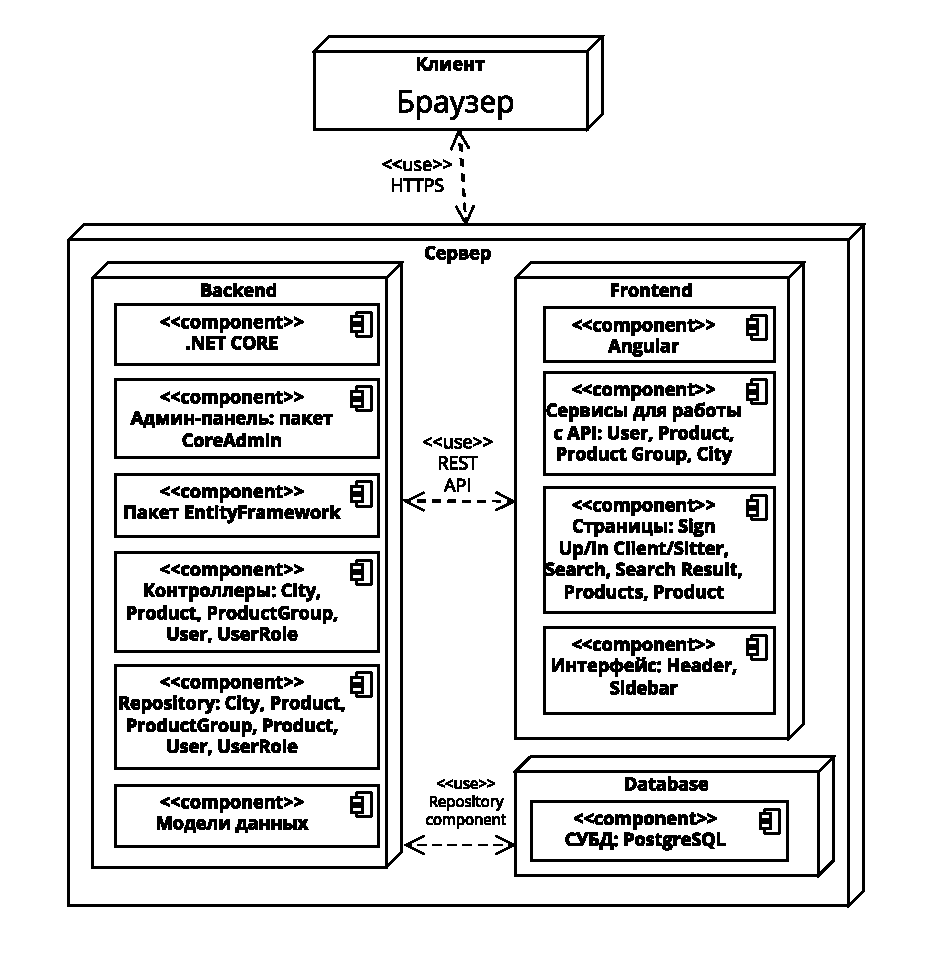
\includegraphics[width=1\linewidth]{client-server.eps}}
\caption{Диаграмма размещения}
\label{place:image}
\end{figure}

Она является хорошим средством для показа маршрутов перемещения объектов и компонентов в распределенной системе.

\subsection{Описание классов системы}

\subsubsection{Описание программных классов серверной части}

\begin{itemize}
    \item <<UserBase>> является фундаментальным классом для хранения пользовательских данных. Помимо основных свойств, таких как <<Phone>>, <<Email>>, <<FirstName>>, <<LastName>>, предлагает основу для дальнейшего расширения и интеграции с другими подсистемами приложения.
    \item <<UserRegistrationData>> расширяет <<UserBase>>, вводя специфические свойства, необходимые для процесса регистрации, включая <<Password>>. Это обеспечивает дополнительный уровень безопасности и индивидуализации данных пользователя.
    \item <<UserLoginData>> применяется для авторизации пользователей в системе. Содержит только самую необходимую информацию для входа, а именно: <<Email>> и <<Password>>.
    \item <<UserLoginResponseData>> и <<UserView>> наследуются от <<UserBase>> и дополняют его уникальным идентификатором <<Id>>. <<UserLoginResponseData>> также включает в себя <<AccessToken>>, что обеспечивает надежную аутентификацию и безопасность данных.
    \item <<User>> представляет собой полную структуру класса пользователя, включая элементы безопасности (<<Hash>> и <<Salt>>) и уникальный идентификатор <<Id>>. Этот класс является центральным в системе управления пользователями и их данными.
\end{itemize}

% Таблица для HashSalt
\begin{xltabular}{\textwidth}{|l|l|p{1.7cm}|X|}
    \caption{Свойства класса <<HashSalt>>}\label{hashsalt_table} \\ \hline
    Свойство & Тип & Обязательное & Описание \\ \hline
    1 & 2 & 3 & 4 \\ \hline
    \endfirsthead
    \caption*{Продолжение таблицы \ref{hashsalt_table}}\\
    1 & 2 & 3 & 4 \\ \hline
    \finishhead
    Hash & String & true & Хэш \\ \hline
    Salt & String & true & Соль для хэша \\ \hline
\end{xltabular}

\newpage

% Таблица для UserBase
\begin{xltabular}{\textwidth}{|l|l|p{1.7cm}|X|}
    \caption{Свойства класса <<UserBase>>}\label{userbase_table} \\ \hline
    Свойство & Тип & Обязательное & Описание \\ \hline
    1 & 2 & 3 & 4 \\ \hline
    \endfirsthead
    \caption*{Продолжение таблицы \ref{userbase_table}}\\
    1 & 2 & 3 & 4 \\ \hline
    \finishhead
    Phone & String & false & Телефонный номер пользователя \\ \hline
    Email & String & false & Электронная почта пользователя \\ \hline
    FirstName & String & false & Имя пользователя \\ \hline
    LastName & String & false & Фамилия пользователя \\ \hline
    ImageUrl & String & false & URL изображения пользователя \\ \hline
    Telegram & String & false & Telegram пользователя \\ \hline
    Website & String & false & Веб-сайт пользователя \\ \hline
\end{xltabular}

\newpage

% Таблица для UserRegistrationData
\begin{xltabular}{\textwidth}{|l|l|p{1.7cm}|X|}
    \caption{Свойства класса <<UserRegistrationData>>}\label{userregdata_table} \\ \hline
    Свойство & Тип & Обязательное & Описание \\ \hline
    1 & 2 & 3 & 4 \\ \hline
    \endfirsthead
    \caption*{Продолжение таблицы \ref{userregdata_table}}\\
    1 & 2 & 3 & 4 \\ \hline
    \finishhead
    Password & String & true & Пароль пользователя \\ \hline
\end{xltabular}

\newpage

% Таблица для UserLoginData
\begin{xltabular}{\textwidth}{|l|l|p{1.7cm}|X|}
    \caption{Свойства класса <<UserLoginData>>}\label{userlogindata_table} \\ \hline
    Свойство & Тип & Обязательное & Описание \\ \hline
    1 & 2 & 3 & 4 \\ \hline
    \endfirsthead
    \caption*{Продолжение таблицы \ref{userlogindata_table}}\\
    1 & 2 & 3 & 4 \\ \hline
    \finishhead
    Email & String & true & Электронная почта пользователя для входа \\ \hline
    Password & String & true & Пароль пользователя для входа \\ \hline
\end{xltabular}

\newpage

% Таблица для UserLoginResponseData
\begin{xltabular}{\textwidth}{|l|l|p{1.7cm}|X|}
    \caption{Свойства класса <<UserLoginResponseData>>}\label{userloginrespdata_table} \\ \hline
    Свойство & Тип & Обязательное & Описание \\ \hline
    1 & 2 & 3 & 4 \\ \hline
    \endfirsthead
    \caption*{Продолжение таблицы \ref{userloginrespdata_table}}\\
    1 & 2 & 3 & 4 \\ \hline
    \finishhead
    Id & Long & true & Уникальный идентификатор пользователя \\ \hline
    AccessToken & String & true & Токен доступа пользователя \\ \hline
\end{xltabular}

\newpage

% Таблица для UserView
\begin{xltabular}{\textwidth}{|l|l|p{1.7cm}|X|}
    \caption{Свойства класса <<UserView>>}\label{userview_table} \\ \hline
    Свойство & Тип & Обязательное & Описание \\ \hline
    1 & 2 & 3 & 4 \\ \hline
    \endfirsthead
    \caption*{Продолжение таблицы \ref{userview_table}}\\
    1 & 2 & 3 & 4 \\ \hline
    \finishhead
    Id & Long & true & Уникальный идентификатор пользователя \\ \hline
\end{xltabular}

\newpage

% Таблица для User
\begin{xltabular}{\textwidth}{|l|l|p{1.7cm}|X|}
    \caption{Свойства класса <<User>>}\label{user_table} \\ \hline
    Свойство & Тип & Обязательное & Описание \\ \hline
    1 & 2 & 3 & 4 \\ \hline
    \endfirsthead
    \caption*{Продолжение таблицы \ref{user_table}}\\
    1 & 2 & 3 & 4 \\ \hline
    \finishhead
    Id & Long & true & Уникальный идентификатор пользователя \\ \hline
    Hash & String & true & Хэш пользователя \\ \hline
    Salt & String & true & Соль для хэша пароля пользователя \\ \hline
\end{xltabular}

Большой набор классов для описания пользователя в серверной части приложение таких как <<UserBase>>, <<UserRegistrationData>>, <<UserLoginData>>, <<UserLoginResponseData>> и <<User>>, подчеркивает разнообразие и сложность структур данных в современных системах. Подход к проектированию и реализации этих классов основывается на объектно-ориентированных принципах и практиках, отмеченных в~\cite{grinchenko} и~\cite{kumskova}.

В частности, класс <<User>> является центральным в системе управления пользователями и их данными, что подчеркивает важность его реализации и интеграции с другими классами.

\newpage

% Таблица для Product
\begin{xltabular}{\textwidth}{|l|l|p{1.7cm}|X|}
    \caption{Свойства класса <<Product>>}\label{product_table} \\ \hline
    Свойство & Тип & Обязательное & Описание \\ \hline
    1 & 2 & 3 & 4 \\ \hline
    \endfirsthead
    \caption*{Продолжение таблицы \ref{product_table}}\\
    1 & 2 & 3 & 4 \\ \hline
    \finishhead
    ImageUrl & String & false & URL изображения продукта \\ \hline
    ProductGroupId & Long & true & Идентификатор группы продуктов \\ \hline
    Price & Float & true & Цена продукта \\ \hline
    Weight & Integer & true & Вес продукта \\ \hline
    CreatedByUserId & Long & true & Идентификатор пользователя, создавшего продукт \\ \hline
\end{xltabular}

\newpage

% Таблица для ProductView
\begin{xltabular}{\textwidth}{|l|l|p{1.7cm}|X|}
    \caption{Свойства класса <<ProductView>>}\label{productview_table} \\ \hline
    Свойство & Тип & Обязательное & Описание \\ \hline
    1 & 2 & 3 & 4 \\ \hline
    \endfirsthead
    \caption*{Продолжение таблицы \ref{productview_table}}\\
    1 & 2 & 3 & 4 \\ \hline
    \finishhead
    CreatedByUser & UserView & true & Пользователь, создавший продукт \\ \hline
\end{xltabular}

\begin{itemize}
    \item <<Product>>, наследующийся от <<Short>>, описывает основные свойства продукта, такие как <<ImageUrl>>, <<ProductGroupId>>, <<Price>>, <<Weight>>, и <<CreatedByUserId>>, указывающий на пользователя, создавшего продукт.
    \item <<ProductView>> расширяет <<Product>>, добавляя <<CreatedByUser>>, который является экземпляром <<UserView>>. Это позволяет получать не только идентификационную информацию о создателе продукта, но и более детальные данные пользователя.
\end{itemize}

\newpage

% Таблица для IUserRepository
\begin{xltabular}{\textwidth}{|l|l|p{1.7cm}|X|}
    \caption{Свойства класса <<IUserRepository>>}\label{iuserrepository_table} \\ \hline
    Свойство & Тип & Обязательное & Описание \\ \hline
    1 & 2 & 3 & 4 \\ \hline
    \endfirsthead
    \caption*{Продолжение таблицы \ref{iuserrepository_table}}\\
    1 & 2 & 3 & 4 \\ \hline
    \finishhead
    GetById & User & true & Получить пользователя по идентификатору \\ \hline
    GetByEmail & User & true & Получить пользователя по электронной почте \\ \hline
    GetAllUserViews & List<UserView> & true & Получить список пользователей \\ \hline
    Create & User & true & Создать пользователя \\ \hline
\end{xltabular}

Класс <<IUserRepository>> описывает основные методы для работы с пользователями, включая получение пользователя по идентификатору, получение пользователя по электронной почте, получение списка пользователей и создание пользователя.

В системе предусмотрен внутренний механизм связи между классами и их свойствами, поэтому введение дополнительных идентификаторов при реализации связей между классами не предполагается.

Экземпляры классов реализуются в информационных блоках посредством элементов, свойства класса – посредством свойств и методов элемента.

\subsubsection{Описание программных классов клиентской части}

\begin{itemize}
    \item <<Short>> - основной класс, используемый для предоставления общей структуры данных. Свойства <<id>>, <<name>> и <<description>> являются фундаментальными для большинства классов;
    \item <<User>> - расширяет <<Short>>, интегрируя контактные данные и личную информацию пользователя. Используется для управления учетными записями пользователей, включая процессы регистрации и авторизации;
    \item <<ProductGroup>> - расширяет <<Short>>, добавляя конкретные детали для организации продуктов в группы. Используется для классификации и управления ассортиментом продуктов;
    \item <<Product>> - расширяет <<Short>>, предоставляя подробную информацию о продуктах. Включает данные о создателе продукта и используется для представления конкретных товаров в системе;
    \item <<City>> - описывает города, со свойствами <<id>> и <<name>>. Используется для управления информацией о местоположениях, связанных с пользователями и продуктами.
    \item <<ProductFilter>> - используется для фильтрации продуктов по городу, группе продуктов, дате публикации и дате окончания срока действия.
\end{itemize}

% Таблица для Short
\begin{xltabular}{\textwidth}{|l|l|p{1.7cm}|X|}
    \caption{Свойства класса <<Short>>\label{int1:table}}\\ \hline
    Свойство & Тип & Обязательное & Описание \\ \hline
    1 & 2 & 3 & 4 \\ \hline
    \endfirsthead
    \caption*{Продолжение таблицы \ref{int1:table}}\\
    1 & 2 & 3 & 4 \\ \hline
    \finishhead
    id & number & true & Уникальный идентификатор \\ \hline
    name & string & true & Название \\ \hline
    description & string & true & Описание \\ \hline
\end{xltabular}

% Таблица для User
\begin{xltabular}{\textwidth}{|l|l|p{1.7cm}|X|}
    \caption{Свойства класса <<User>>\label{int2:table}}\\ \hline
    Свойство & Тип & Обязательное & Описание \\ \hline
    1 & 2 & 3 & 4 \\ \hline
    \endfirsthead
    \caption*{Продолжение таблицы \ref{int2:table}}\\
    1 & 2 & 3 & 4 \\ \hline
    \finishhead
    phone & string & true & Телефонный номер \\ \hline
    email & string & true & Электронная почта \\ \hline
    firstName & string & true & Имя \\ \hline
    lastName & string & true & Фамилия \\ \hline
    photoUrl & string & true & URL изображения \\ \hline
    telegram & string & true & Telegram \\ \hline
    website & string & true & Веб-сайт \\ \hline
    address & string & true & Адрес \\ \hline
    userRoleId & number & true & Идентификатор роли \\ \hline
    password & string & false & Пароль пользователя (передается при авторизации и регистрации) \\ \hline
    accessToken & string & false & Токен доступа (принимается при авторизации и регистрации) \\ \hline
\end{xltabular}

% Таблица для Product
\begin{xltabular}{\textwidth}{|l|l|p{1.7cm}|X|}
    \caption{Свойства класса <<Product>>\label{int3:table}}\\ \hline
    Свойство & Тип & Обязательное & Описание \\ \hline
    1 & 2 & 3 & 4 \\ \hline
    \endfirsthead
    \caption*{Продолжение таблицы \ref{int3:table}}\\
    1 & 2 & 3 & 4 \\ \hline
    \finishhead
    imageUrl & string & true & URL изображения продукта \\ \hline
    productGroupId & number & true & Идентификатор группы продуктов \\ \hline
    price & number & true & Цена продукта \\ \hline
    weight & number & true & Вес продукта \\ \hline
    createdByUserId & number & true & Идентификатор пользователя, создавшего продукт \\ \hline
    publishedAt & Date & true & Дата публикации \\ \hline
    expiredAt & Date & true & Дата окончания срока действия \\ \hline
\end{xltabular}

% Таблица для ProductGroup
\begin{xltabular}{\textwidth}{|l|l|p{1.7cm}|X|}
    \caption{Свойства класса <<ProductGroup>>\label{int4:table}}\\ \hline
    Свойство & Тип & Обязательное & Описание \\ \hline
    1 & 2 & 3 & 4 \\ \hline
    \endfirsthead
    \caption*{Продолжение таблицы \ref{int4:table}}\\
    1 & 2 & 3 & 4 \\ \hline
    \finishhead
    type & string & true & Тип группы продуктов \\ \hline
    childrenProductGroupIds & number[] & true & Идентификаторы дочерних групп продуктов (может быть пустым массивом) \\ \hline
    parentProductGroupId & number & false & Идентификатор родительской группы продуктов \\ \hline
\end{xltabular}

% Таблица для ProductFilter
\begin{xltabular}{\textwidth}{|l|l|p{1.7cm}|X|}
    \caption{Свойства класса <<ProductFilter>>\label{int5:table}}\\ \hline
    Свойство & Тип & Обязательное & Описание \\ \hline
    1 & 2 & 3 & 4 \\ \hline
    \endfirsthead
    \caption*{Продолжение таблицы \ref{int5:table}}\\
    1 & 2 & 3 & 4 \\ \hline
    \finishhead
    cityId & number & false & Идентификатор города \\ \hline
    productGroupId & number & false & Идентификатор группы продуктов \\ \hline
    publishedAtFrom & Date & false & Дата публикации \\ \hline
    expiredAtTo & Date & false & Дата окончания срока действия \\ \hline
\end{xltabular}

% Таблица для City
\begin{xltabular}{\textwidth}{|l|l|p{1.7cm}|X|}
    \caption{Свойства класса <<City>>\label{int6:table}}\\ \hline
    Свойство & Тип & Обязательное & Описание \\ \hline
    1 & 2 & 3 & 4 \\ \hline
    \endfirsthead
    \caption*{Продолжение таблицы \ref{int6:table}}\\
    1 & 2 & 3 & 4 \\ \hline
    \finishhead
    id & number & true & Уникальный идентификатор \\ \hline
    name & string & true & Название города \\ \hline
\end{xltabular}

% Таблица для UserService
\begin{xltabular}{\textwidth}{|l|l|p{1.7cm}|X|}
    \caption{Свойства класса <<UserService>>\label{int6:table}}\\ \hline
    Свойство & Тип & Обязательное & Описание \\ \hline
    1 & 2 & 3 & 4 \\ \hline
    \endfirsthead
    \caption*{Продолжение таблицы \ref{int6:table}}\\
    1 & 2 & 3 & 4 \\ \hline
    \finishhead
    getById & User & true & Получить пользователя по идентификатору \\ \hline
    login & User & true & Получить пользователя по электронной почте \\ \hline
    create & User & true & Получить список пользователей \\ \hline
    update & User & true & Создать пользователя \\ \hline
\end{xltabular}

% Таблица для ProductGroupService
\begin{xltabular}{\textwidth}{|l|l|p{1.7cm}|X|}
    \caption{Свойства класса <<ProductGroupService>>\label{int7:table}}\\ \hline
    Метод & Тип & Обязательное & Описание \\ \hline
    1 & 2 & 3 & 4 \\ \hline
    \endfirsthead
    \caption*{Продолжение таблицы \ref{int7:table}}\\
    1 & 2 & 3 & 4 \\ \hline
    \finishhead
    getAll & ProductGroup[] & true & Получить все группы продуктов \\ \hline
    updateAll & ProductGroup[] & true & Обновить все группы продуктов \\ \hline
\end{xltabular}

% Таблица для ProductService
\begin{xltabular}{\textwidth}{|l|l|p{1.7cm}|X|}
    \caption{Свойства класса <<ProductService>>\label{int8:table}}\\ \hline
    Метод & Тип & Обязательное & Описание \\ \hline
    1 & 2 & 3 & 4 \\ \hline
    \endfirsthead
    \caption*{Продолжение таблицы \ref{int8:table}}\\
    1 & 2 & 3 & 4 \\ \hline
    \finishhead
    getAll & Product[] & true & Получить все продукты \\ \hline
    getById & Product & true & Получить продукт по идентификатору \\ \hline
    add & Product & true & Добавить продукт \\ \hline
    update & Product & true & Обновить продукт \\ \hline
    delete & void & true & Удалить продукт \\ \hline
    getFilteredProducts & Product[] & true & Получить отфильтрованные продукты \\ \hline
\end{xltabular}

% Таблица для CityService
\begin{xltabular}{\textwidth}{|l|l|p{1.7cm}|X|}
    \caption{Свойства класса <<CityService>>\label{int9:table}}\\ \hline
    Метод & Тип & Обязательное & Описание \\ \hline
    1 & 2 & 3 & 4 \\ \hline
    \endfirsthead
    \caption*{Продолжение таблицы \ref{int9:table}}\\
    1 & 2 & 3 & 4 \\ \hline
    \finishhead
    getAll & City[] & true & Получить все города \\ \hline
\end{xltabular}

Классы <<UserService>>, <<ProductGroupService>>, <<ProductService>> и <<CityService>> предоставляют методы для отправки HTTP запросов к API серверной части приложения.
\ifПрактика{}\else{
   \section{Рабочий проект}
\subsection{Классы, используемые при разработке сайта}

Можно выделить следующий список классов и их методов, использованных при разработке web-приложения (таблица \ref{class:table}). Пример таблицы с уменьшенным межстрочным интервалом.

\renewcommand{\arraystretch}{0.8} % уменьшение расстояний до сетки таблицы
\begin{xltabular}{\textwidth}{|X|p{2.5cm}|>{\setlength{\baselineskip}{0.7\baselineskip}}p{4.85cm}|>{\setlength{\baselineskip}{0.7\baselineskip}}p{4.85cm}|}
\caption{Описание классов Bitrix, используемых в приложении\label{class:table}}\\
\hline \centrow \setlength{\baselineskip}{0.7\baselineskip} Название класса & \centrow \setlength{\baselineskip}{0.7\baselineskip} Модуль, к которому относится класс & \centrow Описание класса & \centrow Методы \\
\hline \centrow 1 & \centrow 2 & \centrow 3 & \centrow 4\\ \hline
\endfirsthead
\caption*{Продолжение таблицы \ref{class:table}}\\
\hline \centrow 1 & \centrow 2 & \centrow 3 & \centrow 4\\ \hline
\finishhead
CMain & Главный модуль & CMain – главный класс страницы web-приложения. После одного из этапов по загрузке страницы в сценарии становится доступным инициализированный системой объект данного класса с именем \$APPLICATION & void ShowTitle(string property\_code = «title», bool strip\_tags = true)
Выводит заголовок страницы
void SetTitle(string title)
Устанавливает заголовок страницы

void ShowCSS(bool external = true, bool XhtmlStyle = true)
Выводит таблицу стилей CSS страницы\\
\hline CFile & Главный модуль & CFile – Класс для работы с файлами и изображениями & array GetFileArray (int file\_id)
Метод возвращает массив, содержащий описание файла (путь к файлу, имя файла, размер) с идентификатором file\_id
\end{xltabular}
\renewcommand{\arraystretch}{1.0} % восстановление сетки

\subsection{Модульное тестирование разработанного web-сайта}

Модульный тест для класса User из модели данных представлен на рисунке \ref{unitUser:image}.

\begin{figure}[ht]
\begin{lstlisting}[language=Python]
from django.test import TestCase
from .models import *
User = get_user_model()


class ShpoTestCases(TestCase):

    def setUp(self) -> None:
        self.user = User.objects.create(username='testtestovich', password='testtestovich', first_name='Sad', last_name='')

    def test_2(self):

        self.assertEqual(self.user.first_name, 'Sad')
        self.assertEqual(self.user.last_name, 'Cat')
        print((self.user))
        print((self.user.first_name))
        print((self.user.last_name))
\end{lstlisting}  
\caption{Модульный тест класса User}
\label{unitUser:image}
\end{figure}

\subsection{Системное тестирование разработанного web-сайта}

На рисунке \ref{main:image} представлена главная страница сайта «Русатом – Аддитивные технологии».
\newpage % при необходимости можно переносить рисунок на новую страницу
\begin{figure}[H] % H - рисунок обязательно здесь, или переносится, оставляя пустоту
\center{\includegraphics[width=1\linewidth]{main1}}
\center{\includegraphics[width=1\linewidth]{main2}}
\center{\includegraphics[width=1\linewidth]{main3}}
\caption{Главная страница сайта «Русатом – Аддитивные технологии»}
\label{main:image}
\end{figure}

На рисунке \ref{menu:image} представлен динамический вывод заголовков, включающий в себя искомые фразы при поиске фраз.

\begin{figure}[ht]
\center{\includegraphics[width=1\linewidth]{menu}}
\caption{Динамический вывод заголовков}
\label{menu:image}
\end{figure}

На рисунке \ref{enter:image} представлен ввод данных для публикации новости.

\begin{figure}[ht]
\center{\includegraphics[width=1\linewidth]{enter}}
\caption{Ввод данных для публикации очень-очень длинной, интересной и полезной новости}
\label{enter:image}
\end{figure}

   \section*{ЗАКЛЮЧЕНИЕ}
\addcontentsline{toc}{section}{ЗАКЛЮЧЕНИЕ}

Преимущества аддитивных технологий заключается в разнообразии процессов, позволяющих применять их в различных областях производства. Существенным ограничением же является и экономическая составляющая, которая не позволит внедрить аддитивное производство повсеместно.
  
Компании, видя, как развиваются информационные технологии, пытаются использовать их выгодно для своего бизнеса, запуская свой сайт для того, чтобы заявить о своем существовании, проинформировать потенциального клиента об услугах или продуктах, которые предоставляет. 
Для продвижения компании «Русатом – Аддитивные технологии» был разработан веб-сайт на основе системы «1С-Битрикс: Управление сайтом».

Основные результаты работы:

\begin{enumerate}
\item Проведен анализ предметной области. Выявлена необходимость использовать 1С-Битрикс.
\item Разработана концептуальная модель web-сайта. Разработана модель данных системы. Определены требования к системе.
\item Осуществлено проектирование web-сайта. Разработана архитектура серверной части. Разработан пользовательский интерфейс web-сайта.
\item Реализован и протестирован web-сайт. Проведено модульное и системное тестирование.
\end{enumerate}

Все требования, объявленные в техническом задании, были полностью реализованы, все задачи, поставленные в начале разработки проекта, были также решены.

Готовый рабочий проект представлен адаптивной версткой сайта. Сайт находится в публичном доступе, поскольку опубликован в сети Интернет.  

}\fi
% \addcontentsline{toc}{section}{СПИСОК ИСПОЛЬЗОВАННЫХ ИСТОЧНИКОВ}
%
% \begin{thebibliography}{9}
%
%     \bibitem{javascript} Фримен, А. Практикум по программированию на JavaScript / А. Фримен. – Москва : Вильямс, 2013. – 960 с. – ISBN 978-5-8459-1799-7. – Текст : непосредственный.
%     \bibitem{php} Бретт, М. PHP и MySQL. Исчерпывающее руководство / М. Бретт. – Санкт-Петербург : Питер, 2016. – 544 с. – ISBN 978-5-496-01049-8. – Текст : непосредственный.
%     \bibitem{css} Веру, Л. Секреты CSS. Идеальные решения ежедневных задач / Л. Веру. – Санкт-Петербург : Питер, 2016. – 336 с. – ISBN 978-5-496-02082-4. – Текст : непосредственный.
%     \bibitem{mysql}	Гизберт, Д. PHP и MySQL / Д. Гизберт. – Москва : НТ Пресс, 2013. – 320 с. – ISBN 978-5-477-01174-2. – Текст : непосредственный.
% 	\bibitem{html5}	Голдстайн, А. HTML5 и CSS3 для всех / А. Голдстайн, Л. Лазарис, Э. Уэйл. – Москва : Вильямс, 2012. – 368 с. – ISBN 978-5-699-57580-0. – Текст : непосредственный.
% 	\bibitem{htmlcss}	Дэкетт, Д. HTML и CSS. Разработка и создание веб-сайтов / Д. Дэкетт. – Москва : Эксмо, 2014. – 480 с. – ISBN 978-5-699-64193-2. – Текст : непосредственный.
% 	\bibitem{bigbook}	Макфарланд, Д. Большая книга CSS / Д. Макфарланд. – Санкт-Петербург : Питер, 2012. – 560 с. – ISBN 978-5-496-02080-0. – Текст : непосредственный.
% 	\bibitem{uchiru}	Лоусон, Б. Изучаем HTML5. Библиотека специалиста / Б. Лоусон, Р. Шарп. – Санкт-Петербург : Питер, 2013 – 286 с. – ISBN 978-5-459-01156-2. – Текст : непосредственный.
% 	\bibitem{chaynik}	Титтел, Э. HTML5 и CSS3 для чайников / Э. Титтел, К. Минник. – Москва : Вильямс, 2016 – 400 с. – ISBN 978-1-118-65720-1. – Текст : непосредственный.
% 	\bibitem{22}	Титтел, Э. HTML5 и CSS3 для чайников / Э. Титтел, К. Минник. – Москва : Вильямс, 2016 – 400 с. – ISBN 978-1-118-65720-1. – Текст : непосредственный.
% 	\bibitem{1231}	Титтел, Э. HTML5 и CSS3 для чайников / Э. Титтел, К. Минник. – Москва : Вильямс, 2016 – 400 с. – ISBN 978-1-118-65720-1. – Текст : непосредственный.
% 	\bibitem{sdf}	Титтел, Э. HTML5 и CSS3 для чайников / Э. Титтел, К. Минник. – Москва : Вильямс, 2016 – 400 с. – ISBN 978-1-118-65720-1. – Текст : непосредственный.
% 	\bibitem{servsssds}	Титтел, Э. HTML5 и CSS3 для чайников / Э. Титтел, К. Минник. – Москва : Вильямс, 2016 – 400 с. – ISBN 978-1-118-65720-1. – Текст : непосредственный.
% \end{thebibliography}
\addcontentsline{toc}{section}{СПИСОК ИСПОЛЬЗОВАННЫХ ИСТОЧНИКОВ}

\begin{thebibliography}{20}
    \bibitem{market} Герасимов, Н.Н. Маркетинговые исследования рынка. Учебное пособие. / Б.И. Герасимов, Н.Н. Мозгов. – Москва : Форум, 2014. – 336 с. ISBN978-5-91134-811-3. – Текст : непосредственный.

    \bibitem{yordon} Йордон, Э. Путь камикадзе. Как разработчику программного обеспечения выжить в безнадежном проекте / Эдвард Йордон. – Москва : Лори, 2019. – 256 с. – ISBN 978-5-124840-1. – Текст : непосредственный.%TODO настоящий ISBN

    \bibitem{averin} Аверин, А.В. Стандартизация и регламентация государственных услуг : Российский и зарубежный опыт / А.В. Аверин. – Москва : Урал, 2015. – с. 727. – ISBN 978-5-124840-1. – Текст : непосредственный.%TODO настоящий ISBN

    \bibitem{grinchenko} Гринченко, Н.Н. Проектирование баз данных. СУБД Microsoft Ассеss : Учебное пособие для вузов / Н.Н. Гринченко и др. – Москва : РиС, 2013. – 240 с. – ISBN 978-5-592-340-52. – Текст : непосредственный.%TODO настоящий ISBN

    \bibitem{postgresql} Postgresql.org -\- Документация базы данных : сайт. - URL : https ://www.postgresql.org/docs/ (дата обращения : 20.05.2022). - Текст : электронный.

    \bibitem{makni} Макни, Дж.К. Проектирование серверной инфраструктуры баз данных Microsoft SQL Server 2005 / Дж.К. Макни. – Москва : Русская редакция, 2008. – 560 с. – ISBN 978-5-148180-9. – Текст : непосредственный.%TODO настоящий ISBN

    \bibitem{cssspecs} W3C Specifications -\- спецификация CSS : сайт. – URL : https ://www.w3.org/Style/CSS/specs.en.html (дата обращения : 20.12.2023). – Текст : электронный.

    \bibitem{htmlbook} HTMLBOOK -\- спецификация НТМL : сайт. - URL : http ://htmlbook.ru/html (дата обращения : 10.12.2023). - Текст : электронный.

 	\bibitem{html5}	Голдстайн, А. HTML5 и CSS3 для всех / А. Голдстайн, Л. Лазарис, Э. Уэйл. – Москва : Вильямс, 2012. – 368 с. – ISBN 978-5-699-57580-0. – Текст : непосредственный.

    \bibitem{boyko} Бойко, И. Объектно-ориентированные СУБД / И. Бойко. – Киев : Высшая школа, 2014. – ISBN 978-5-489-5120-0. – Текст : непосредственный.%TODO настоящий ISBN

    \bibitem{kumskova} Кумскова, И.А. Базы данных. Учебник для ССУЗов / И.А. Кумскова. – Москва : КноРус, 2012. – 488 с. – ISBN 978-5-182921-8. – Текст : непосредственный.%TODO настоящий ISBN

    \bibitem{mark_price} Прайс, М. C\# 9 и .NET 5. Разработка и оптимизация / Марк Прайс. – Санкт-Петербург : Питер, 2021. – 832 с. – ISBN 978-5-4461-2921-8. – Текст : непосредственный.

    \bibitem{msdn} MSDN -\- сеть разработчиков Microsoft. URL : https ://msdn.microsoft.com (дата обращения : 22.12.2023). – Текст : электронный.

    \bibitem{stackoverflow} StackOverflow -\- сайт вопросов и ответов для программистов. URL : https ://ru.stackoverflow.com/ (дата обращения : 10.01.2024). – Текст : электронный.

    \bibitem{freeman} Фримен, Э. Изучаем Angular : Руководство по созданию приложений на Angular / Эрик Фримен, Элизабет Робсон. – Москва : Эксмо, 2018. – 720 с. – ISBN 978-5-699-98165-6. – Текст : непосредственный.

    \bibitem{troelsen} Троелсен, Э. Язык программирования C\# 7 и платформы .NET и .NET Core / Эндрю Троелсен, Филип Джепикс. – Москва : Вильямс, 2018. – 1456 с. – ISBN 978-5-8459-2114-9. – Текст : непосредственный.

    \bibitem{freedman} Фридман, Д. Методы исследования рынков / Дэвид Фридман, Сэм Либерман. – Москва : Альпина Паблишер, 2016. – 560 с. – ISBN 978-5-9614-5403-5. – Текст : непосредственный.

    \bibitem{riccardi} Риккарди, Дж. ASP.NET Core 6 : Современное развитие веб-приложений на C\# / Джейсон Риккарди. – Москва : ДМК Пресс, 2022. – 512 с. – ISBN 978-5-97060-837-9. – Текст : непосредственный.

    \bibitem{kofman} Кофман, Л. Паттерны проектирования для эффективной работы с базами данных : EF Core / Леонид Кофман. – Москва : Рид Групп, 2020. – 336 с. – ISBN 978-5-496-03125-3. – Текст : непосредственный.

    \bibitem{rxjs} Атенсио, Л. Функциональное программирование на JavaScript / Л. Атенсио – Москва : Диалектика, 2018. – 306 с. – ISBN 978-5-9909445-8-9. – Текст : непосредственный.

\end{thebibliography}

\ifВКР{\appendix{Представление графического материала}

Графический материал, выполненный на отдельных листах,
изображен на рисунках А.1--А.10.

\renewcommand{\thefigure}{А.\arabic{figure}} % шаблон номера для плакатов

\begin{плакат}
    
\includegraphics[width=1.3\linewidth]{плакат1.png}
    \заголовок{Сведения о ВКРБ}
    \label{pl1:image}      
\end{плакат}

\begin{плакат}
    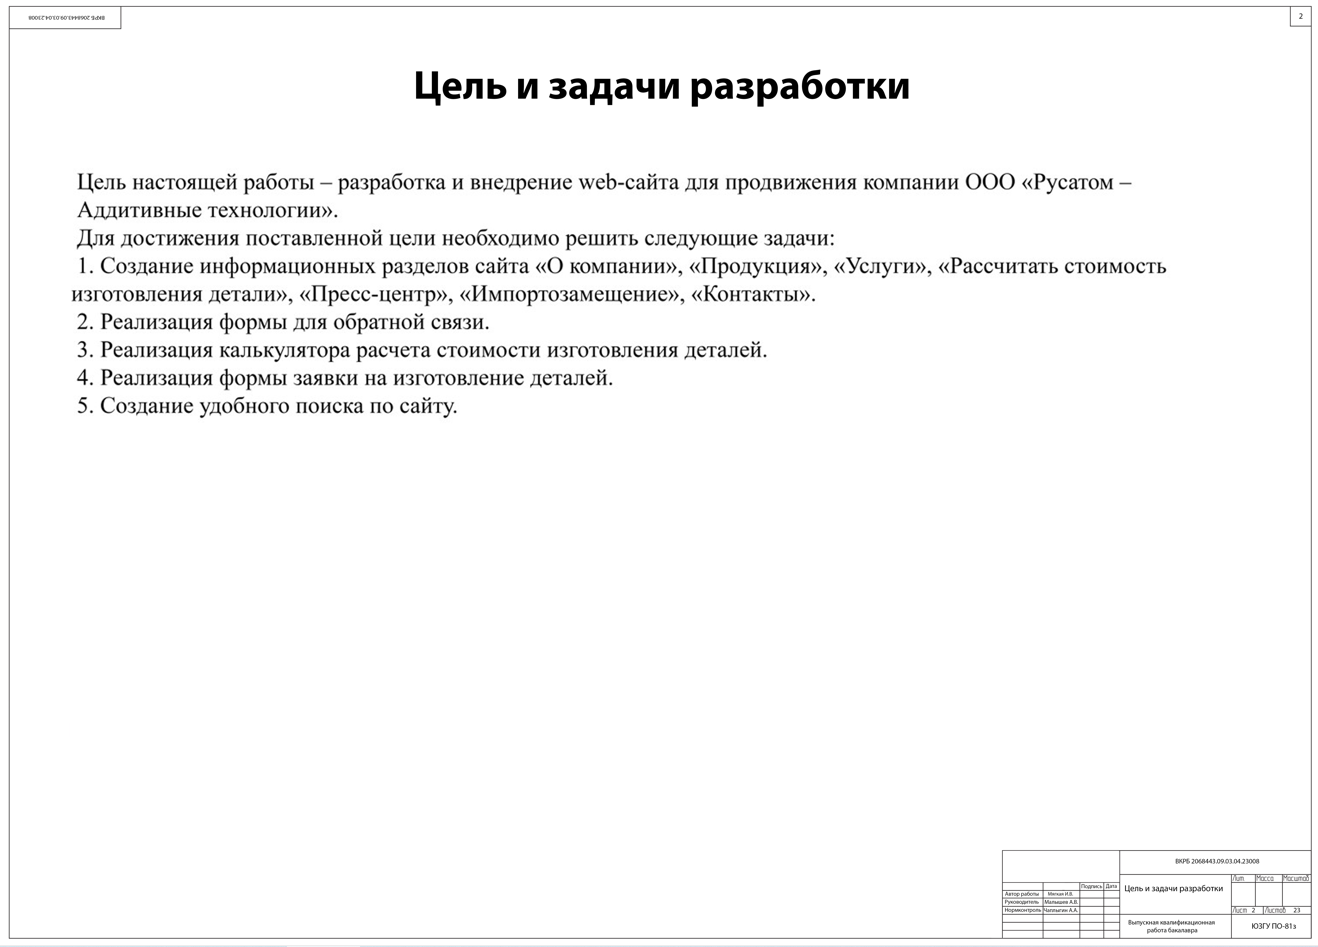
\includegraphics[width=1.3\linewidth]{плакат2.png}
    \заголовок{Цель и задачи разработки}
    \label{pl2:image}      
\end{плакат}

\begin{плакат}
    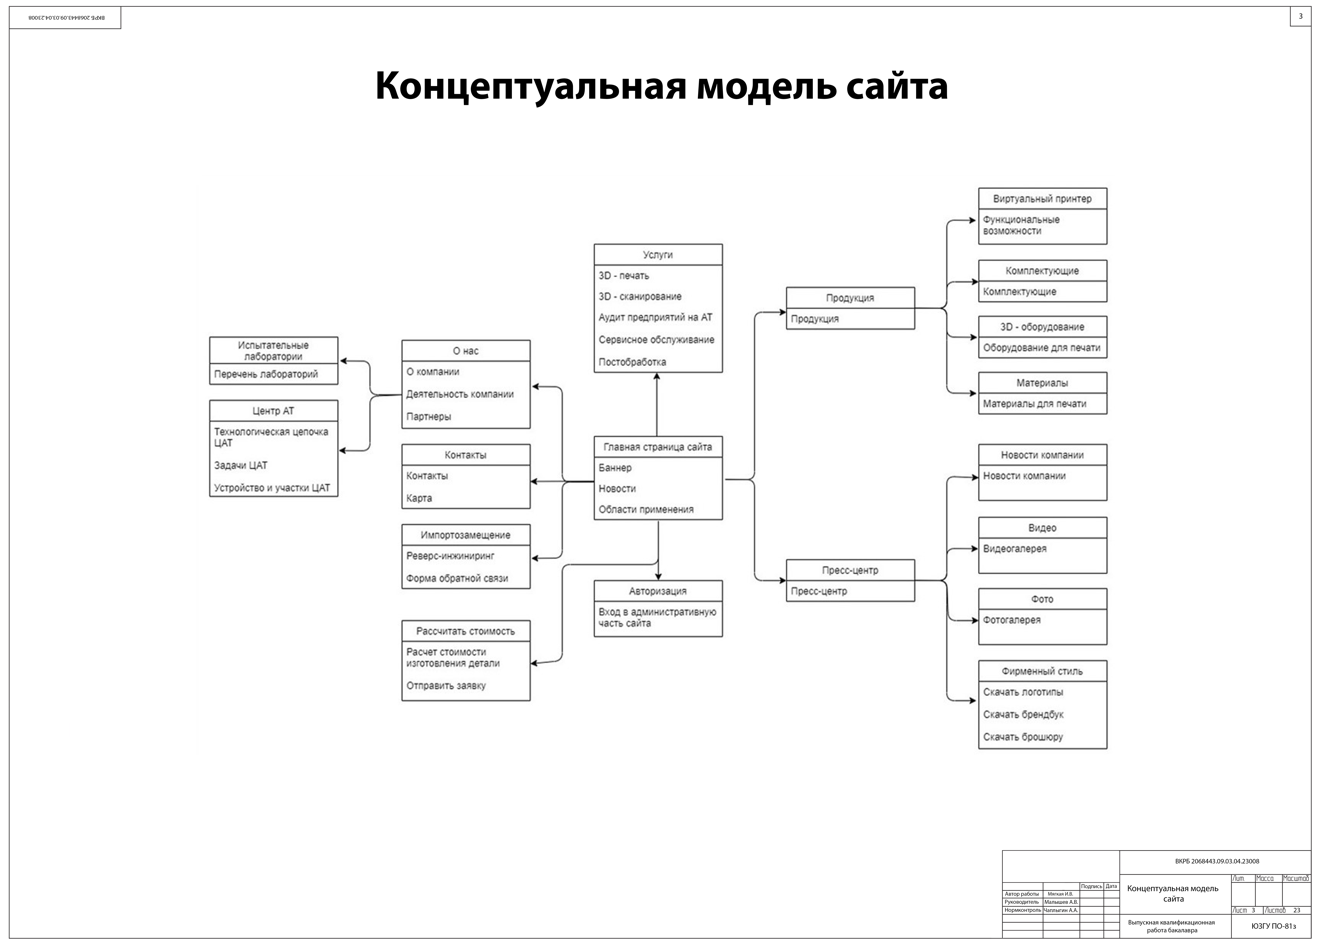
\includegraphics[width=1.3\linewidth]{плакат3.png}
    \заголовок{Концептуальная модель сайта}
    \label{pl3:image}      
\end{плакат}

%\begin{figure}
%  \begin{adjustbox}{addcode={\begin{minipage}{\width}}{\caption{%
%          Сведения о ВКРБ
%      }\end{minipage}},rotate=90,center}
%    
\includegraphics[width=1.3\linewidth]{плакат1.png}
%  \end{adjustbox}
%  \label{pl1:image}      
%\end{figure}

%\begin{figure}
%  \begin{adjustbox}{addcode={\begin{minipage}{\width}}{\caption{%
%          Цель и задачи разработки
%      }\end{minipage}},rotate=90,center}
%    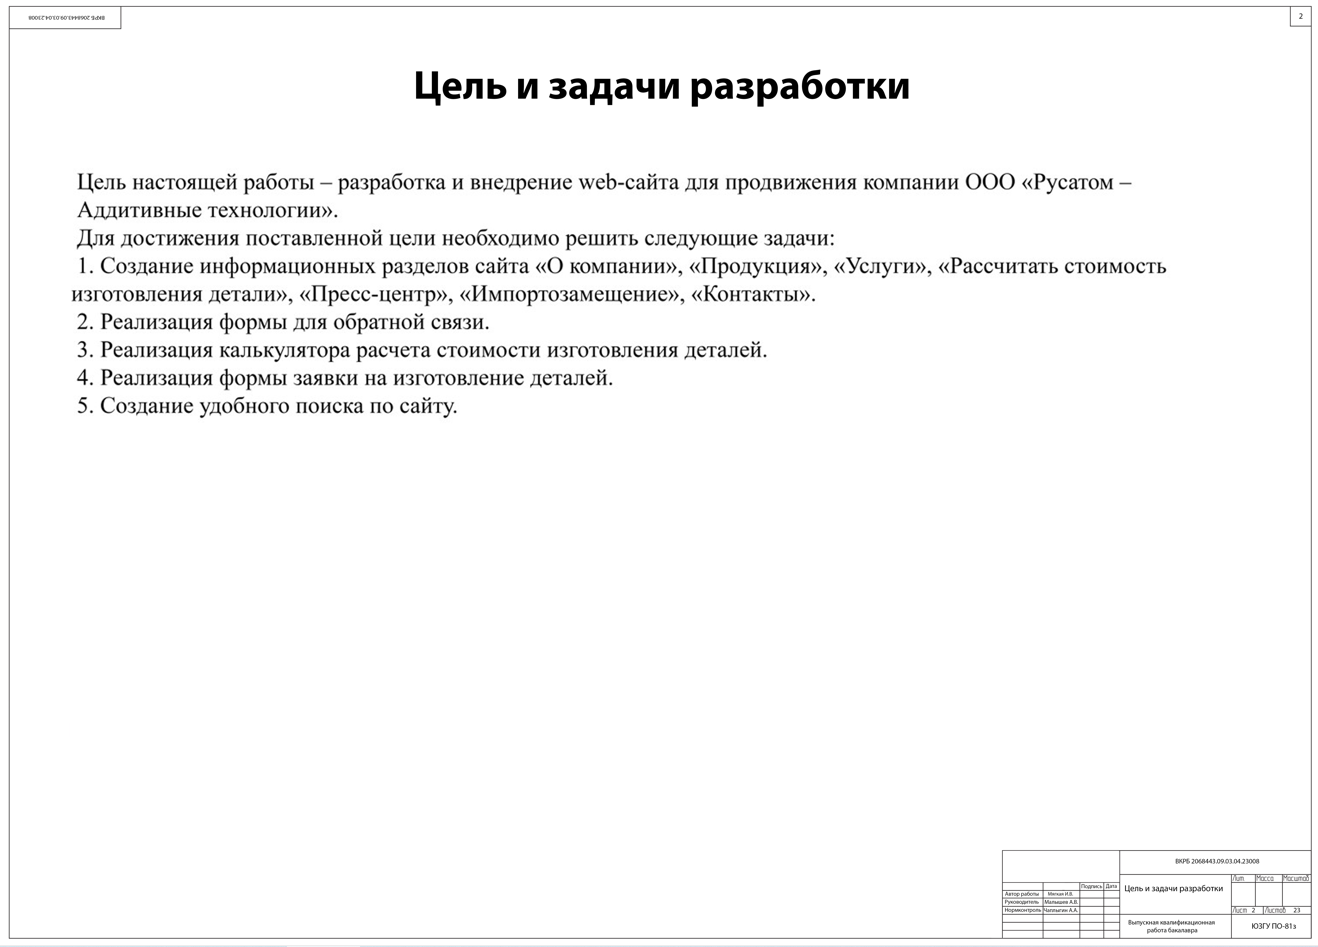
\includegraphics[width=1.3\linewidth]{плакат2.png}
%  \end{adjustbox}
%  \label{pl2:image}      
%\end{figure}

%\begin{figure}
%  \begin{adjustbox}{addcode={\begin{minipage}{\width}}{\caption{%
%          Концептуальная модель сайта
%      }\end{minipage}},rotate=90,center}
%    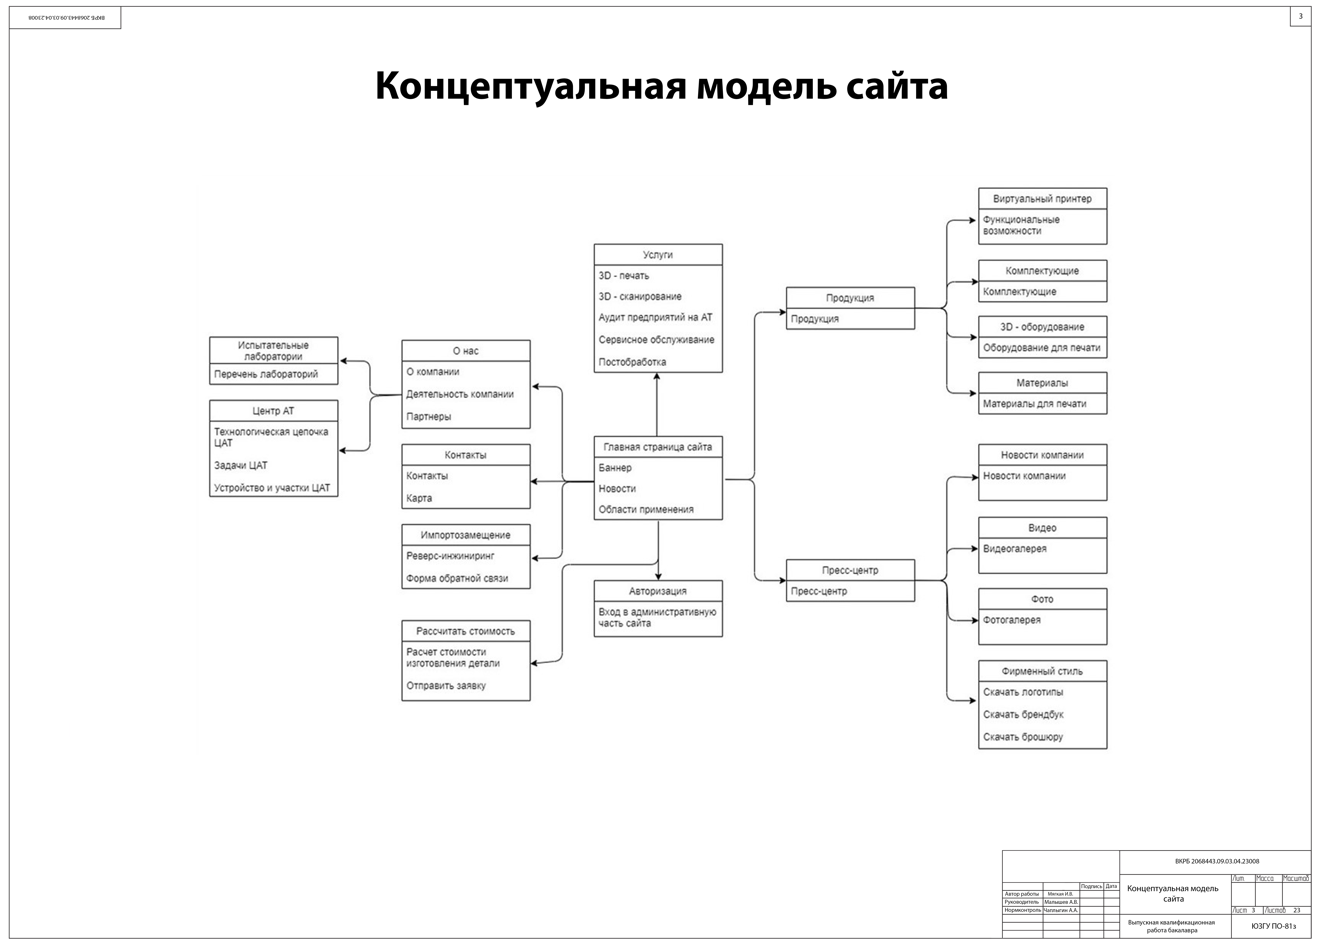
\includegraphics[width=1.3\linewidth]{плакат3.png}
%  \end{adjustbox}
%  \label{pl3:image}      
%\end{figure}
}\fi
\ifПрактика{}\else{\appendix{Фрагменты исходного кода программы}\applabel{Код}

main.tex
\lstinputlisting[language=Tex, frame=none]{main.tex}

ТехПроект.tex
\lstinputlisting[language=Tex, frame=none]{ТехПроект.tex}

\newpage
\addcontentsline{toc}{section}{На отдельных листах (CD-RW в прикрепленном конверте)}

\begin{center}
\textbf{Место для диска}
\end{center}
}\fi
\end{document}
